\chapter{Fitting}
The parameters of interest are extracted from the data samples via an extended unbinned maximum likelihood fit to the dimuon invariant-mass spectra.
In this section, the fitter study is carried out for two selected $p_{T}^{\mu}$ cut, 3.5 and 4.0 $\GeVc$. 
But the final results in Section~\ref{sec:dooubleratio} is given with the nominal 4.0 $\GeVc$ cut only. 
The baseline fitting model is improved relative to the publication using the 2010 dataset. We explored complementary approaches for background modeling (eg employing like-sign parameterizations, track rotation).
%

The baseline fitting model is inspired in that used in~\cite{CMS_AN_2010-140, CMS_AN_2011_062}. 
%
Each of the $\PgU$(nS) signals is modeled via a crystal-ball shape (CB), 
which consists of a Gaussian function with the low-side tail replaced with a power law describing final-state radiation (FSR). 
%
The crystal-ball function is given by:
%
\begin{linenomath}
\begin{equation}
  f(x;\alpha,n,\bar x,\sigma) = N \cdot \left\{
  \begin{array}{ll}
    \exp(- \frac{(x -\bar x)^2}{2 \sigma^2})      & \mbox{for } \frac{x - \bar x}{\sigma} > -\alpha \\ 
    A \cdot (B - \frac{x - \bar x}{\sigma})^{-n}  & \mbox{for } \frac{x - \bar x}{\sigma} \leq -\alpha \,,
  \end{array} 
  \right.
\end{equation}
\end{linenomath}
%
where 
\begin{linenomath}
\begin{eqnarray}
  A & = & \left(\frac{n}{\left| \alpha \right|}\right)^n \cdot \exp\left(- \frac {\left| \alpha \right|^2}{2}\right) \,, \nonumber \\
  B & = & \frac{n}{\left| \alpha \right|} - \left| \alpha \right| \,. \nonumber
\end{eqnarray}
\end{linenomath}
%
The CB function is parameterized by four parameters -- the mass mean $\bar x$ and resolution $\sigma$, and the tail parameters $\alpha$ and $n$ -- which are constrained amongst the three signal peaks:    
the tail parameters are common; 
the resolution  forced to scale with the resonance mass;  
the differences of the mass means are fixed to their PDG values. % ($\Delta_{12}=563\MeVcc$, $\Delta_{13}=332\MeVcc$). 

%The floating fit parameters are the resonance yield and/or yield-ratios, the $\PgUa$ mass, and all of the background parameters. The fits to the pp and PbPb data are shown in \fig{fig:ups_pp_and_PbPb_separate} 

In the previous iteration of the analysis~\cite{prl}, based on the 2010 dataset, 
the signal PDF shape parameters were fixed from MC simulation: $\alpha=1.6$, $n=2.3$, $\sigma_{1S}=92\MeVcc$. 
%
In view of the larger dataset currently available, such constraints have been relaxed. %, based on the studies documented next.  
Specifically, the following signal shape parameters are free in the fit:
the $\PgUa$ mass mean and resolution, the tail parameter $\alpha$.
Note that, given $\alpha$ and $n$ are strongly correlated, the constraint $n=2.3$ is kept in the fit. 


The $\pt$ threshold applied for muon selection induces a sculpting of the mass background distribution, as described in Section~\ref{sec:shoulder}.  
%\emph{(add reference to the relevant section in the selection chapter)}. 
The background parameterization adopted corresponds to an exponential function (exp), multiplied by an error-function (erf), where the latter describes the induced kinematic shoulder and is defined as:
%
\begin{linenomath}
\begin{equation}
\mbox{erf}(x)=\frac{2}{\sqrt{\pi}}\int_0^x e^{-t^2} \: dt
\end{equation}
\end{linenomath}
%
The background model is thus described by three parameters: the exponential decay constant, and the turn-on mean and width. All background parameters are left free. % for the nominal $\pt>3.5 \GeVc$ selection. 
%For the  $\pt>4.0 \GeVc$ case, the shoulder is located within the signal region, and the error-function parameters need to be constrained -- in this case, the background peaks under the signal peak, and the fit cannot reliably descriminate signal from background for events under the CB tail. 

The nominal fit results to the PbPb data are shown in \fig{fig:massfit_nominal_all}. 
%
% https://espace.cern.ch/cms-heavyion/upsilon/fitting/errorFunction_70microb.aspx
%
\begin{figure}[hbtp]
  \begin{center}
    \subfigure[$\pt^\mu>3.5\GeVc$]{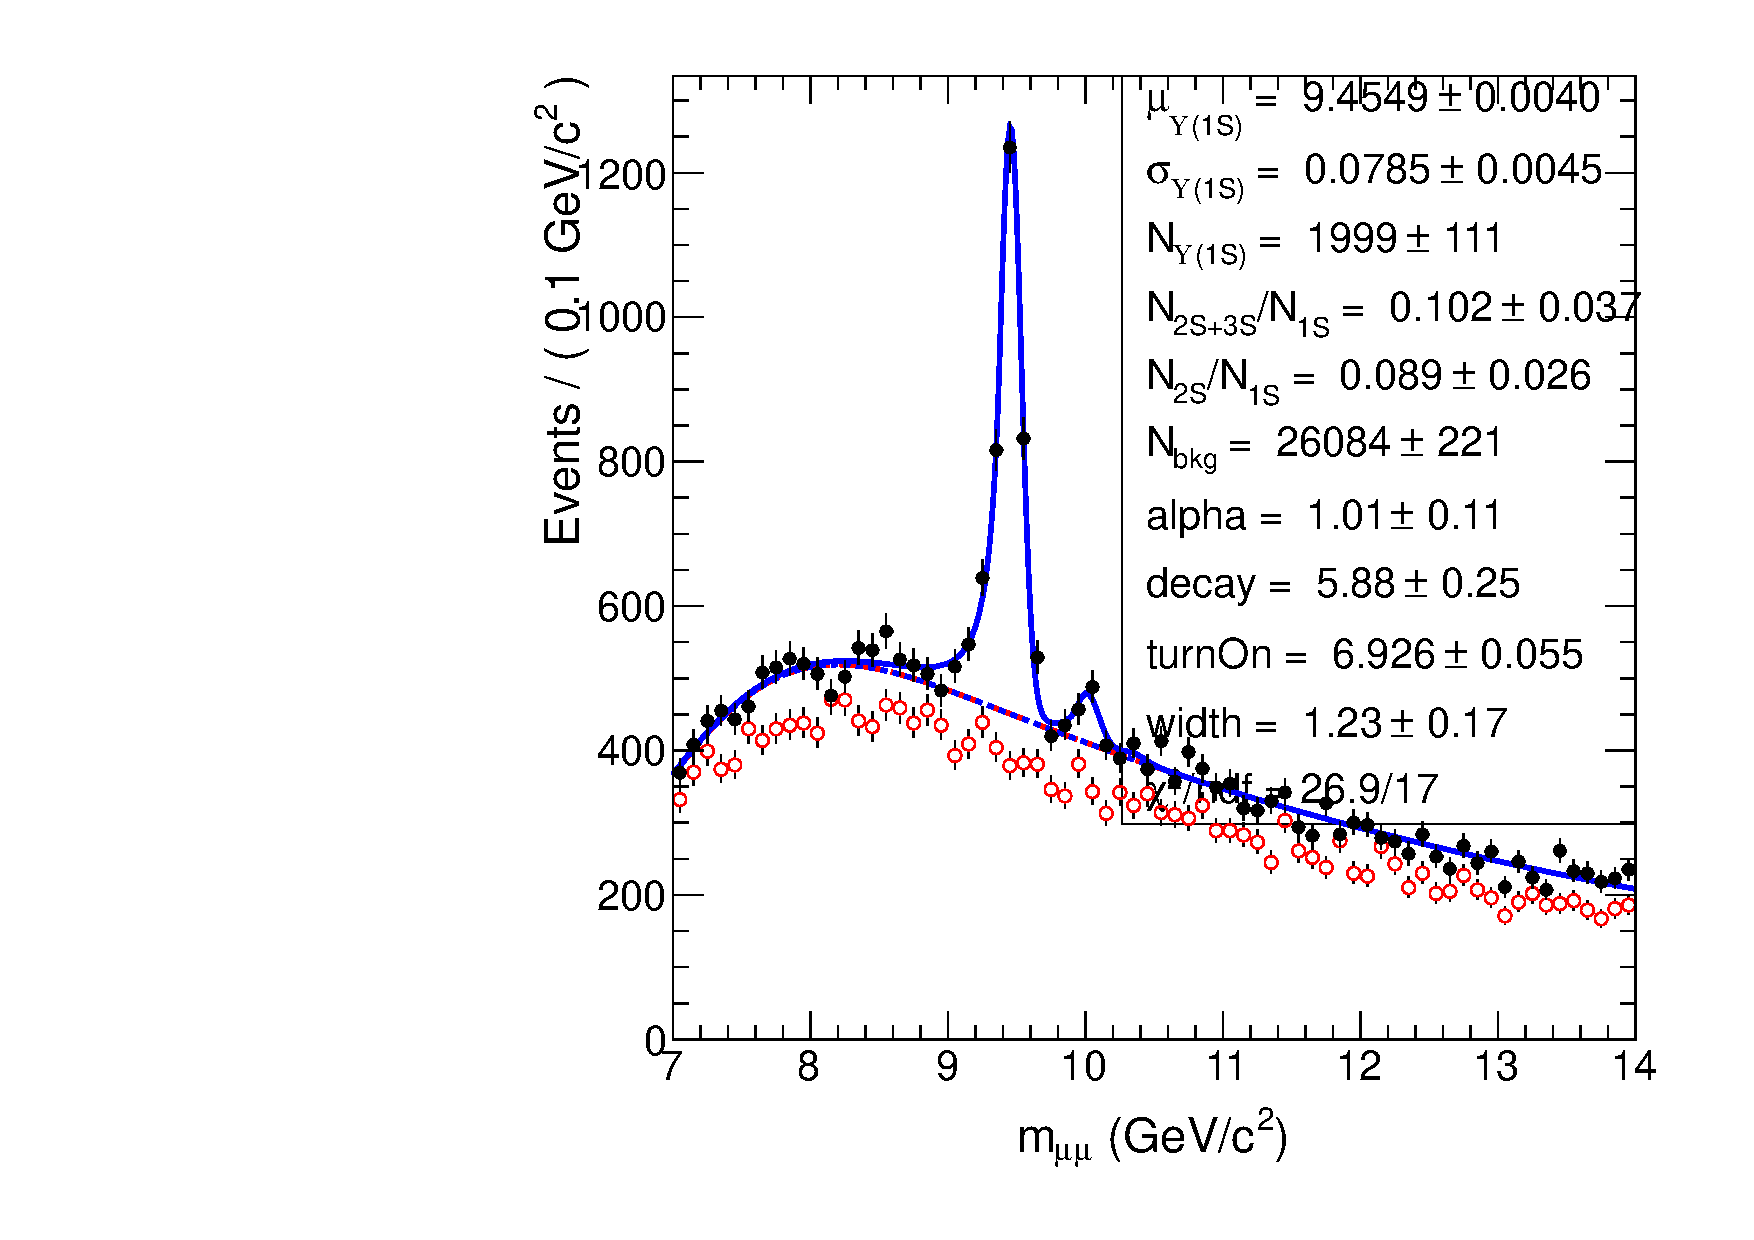
\includegraphics[angle=0,width=0.5\textwidth]{figures/fitting/masspeak_Hi_paramOn_MuonPT35_150imub}}
    \subfigure[$\pt^\mu>4.0\GeVc$]{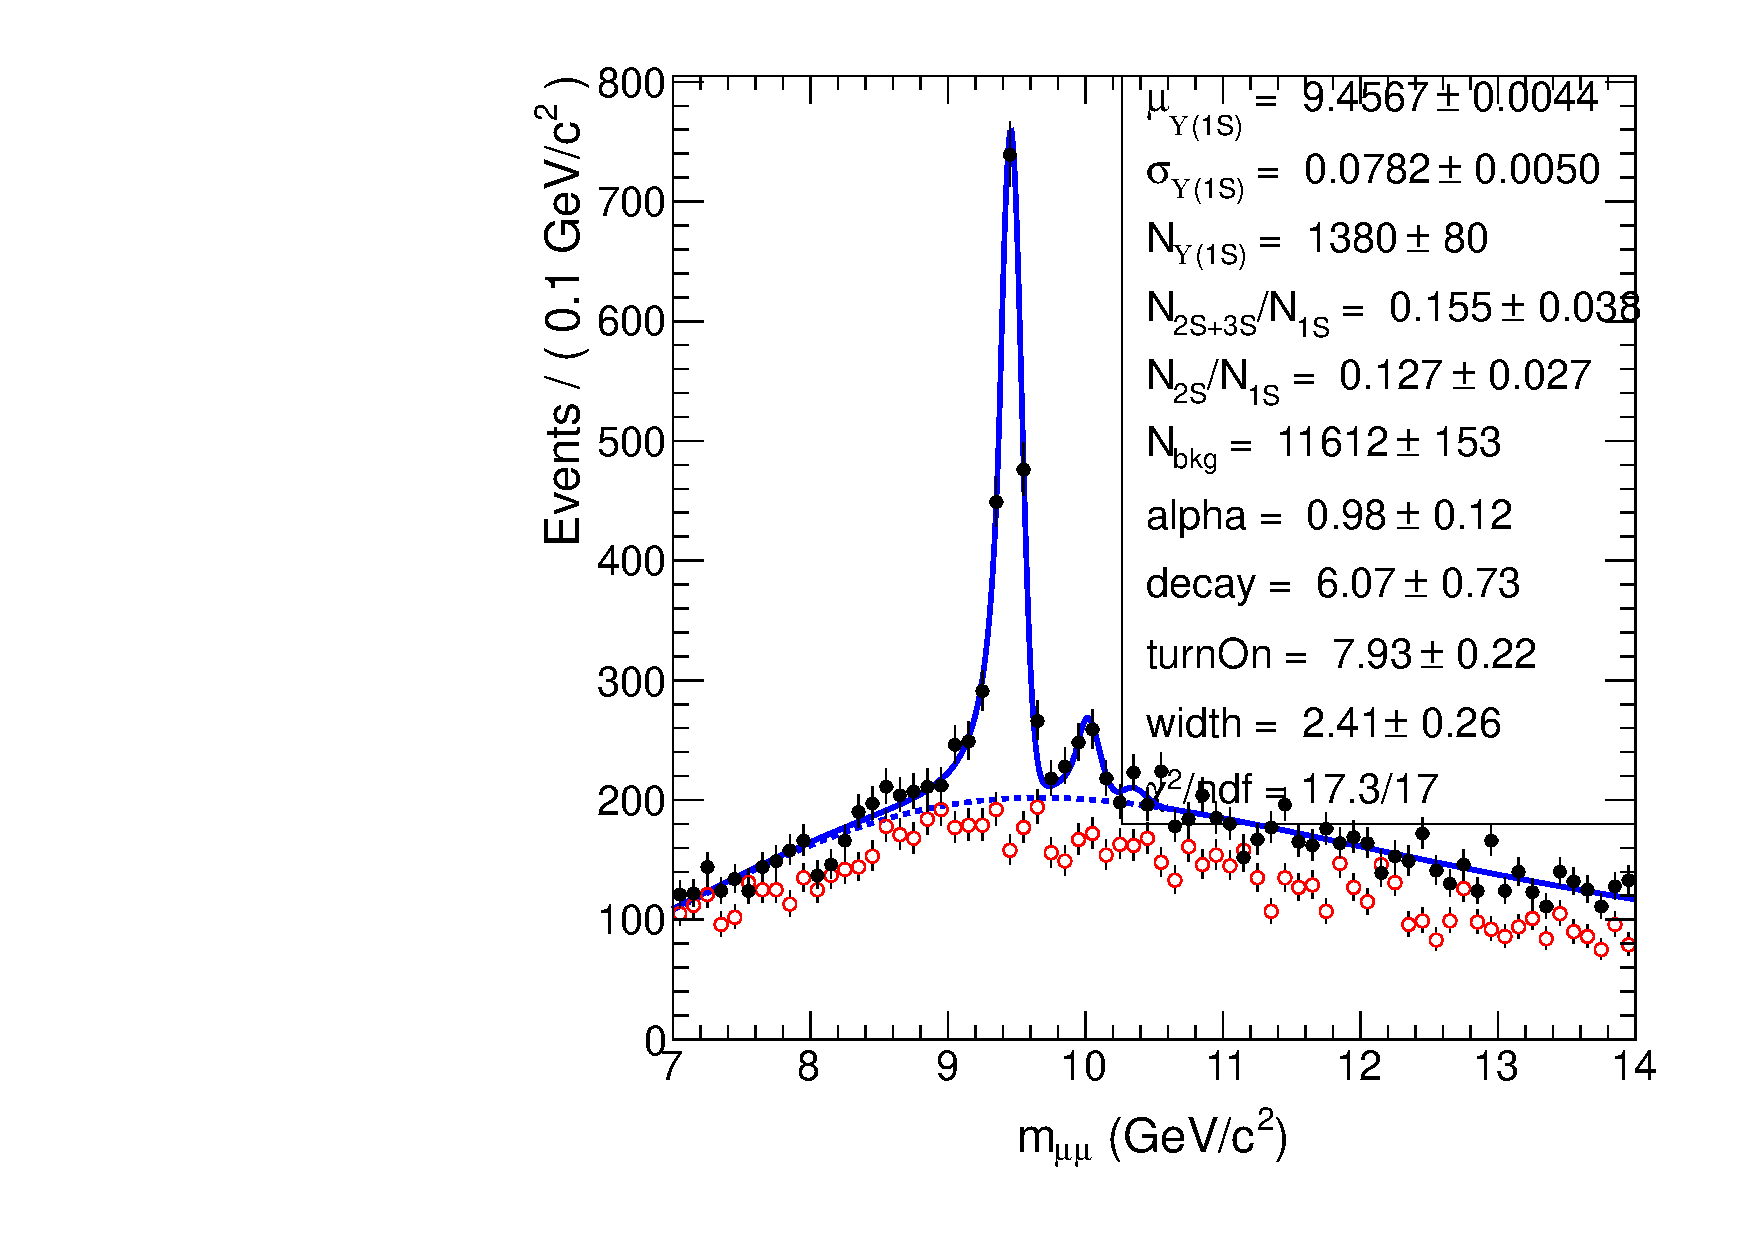
\includegraphics[angle=0,width=0.5\textwidth]{figures/fitting/masspeak_Hi_paramOn_MuonPT4_150imub}}\label{fig:massfit_nominal}
  \caption{Fit to the dimuon invariant-mass distributions, for the PbPb sample. ($150 \mu b^{-1}$) }
  \label{fig:massfit_nominal_all}
  \end{center}
\end{figure}

\subsection{Signal model studies}


\subsubsection{Final state radiation model}

% https://espace.cern.ch/cms-heavyion/upsilon/fitting/RadiationTailFromMC.aspx

We first estimate the CB tail from Monte Carlo simulation of final state radiation. % (enter reference for Photos / EvtGen interface to Pythia). 
The MC sample is first split in multiple (about 50) sub-samples, of statistics comparable to data. These samples are fitted in turn, and the average parameter values are determined. This is shown in~\fig{fig:fsr_mc_pull}. 
%The values obtained are ... No!: let;s avoid having too many numbers spread in the text, which we will not be able to "maintain" -- instead summarize numbers in tables only
 
\begin{figure}[hbtp]
  \begin{center}
    \subfigure[fixed: $\sigma = 92 \MeVcc$, $n=2.3$; float: $\alpha$  ]{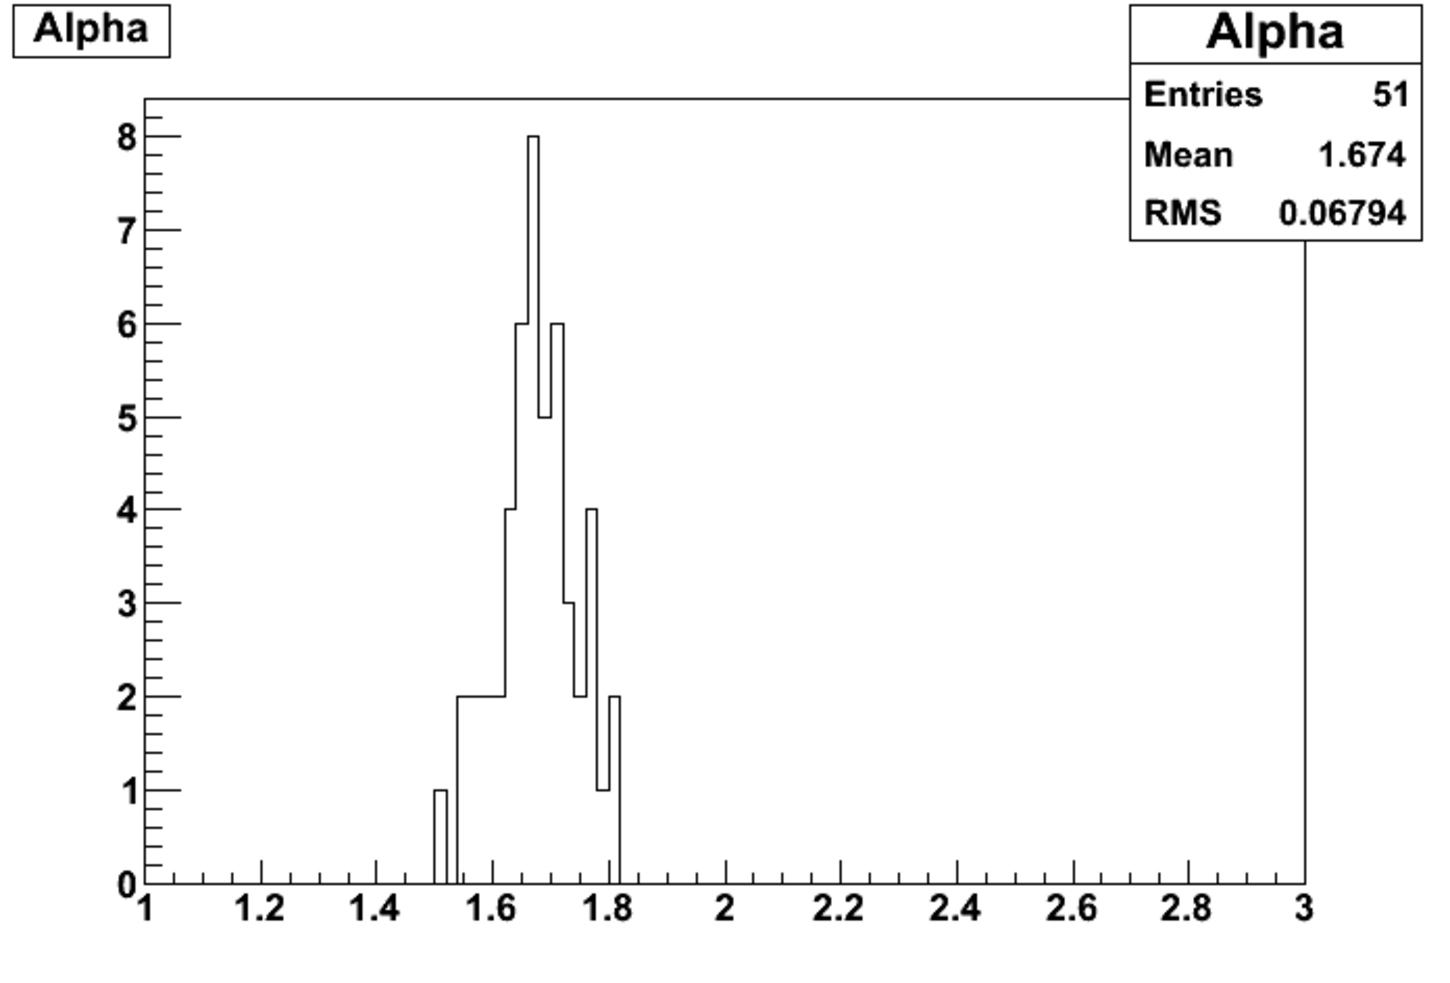
\includegraphics[angle=0,width=0.5\textwidth]{figures/fitting/mc_fsr_mean_alpha.pdf}}
    \subfigure[fixed: $\sigma = 92 \MeVcc$, $\alpha=1.674$; float: $n$]{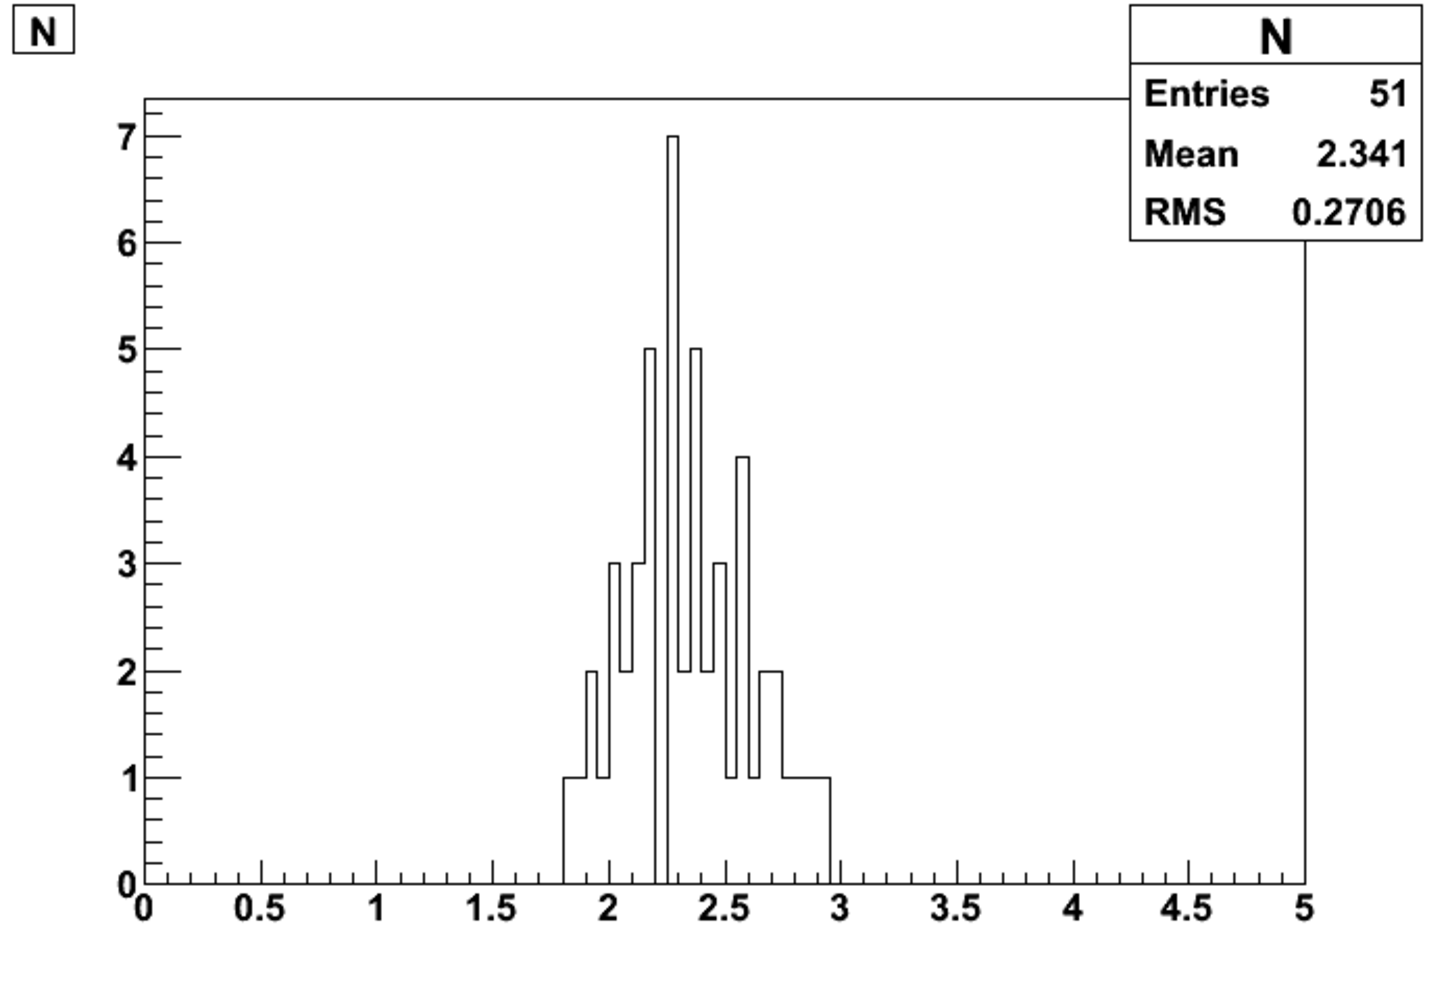
\includegraphics[angle=0,width=0.5\textwidth]{figures/fitting/mc_fsr_mean_n.pdf}}
  \caption{FSR parameter estimation from MC.}
  \label{fig:fsr_mc_pull}
  \end{center}
\end{figure}

For estimating the CB tail from data, the fit is performed after subtracting the  like-sign dimuon mass distribution. This procedure results in a mostly flat remaining background. In this way, the (binned) fit to the subtracted data is able to better constrain the background shape from the mass side-bands, allowing also a more reliable determination of the CB tail. Fit examples are shown in~\fig{fig:fsr_data_bins}. 


\begin{figure}[hbtp]
  \begin{center}
    \subfigure[bins:100]{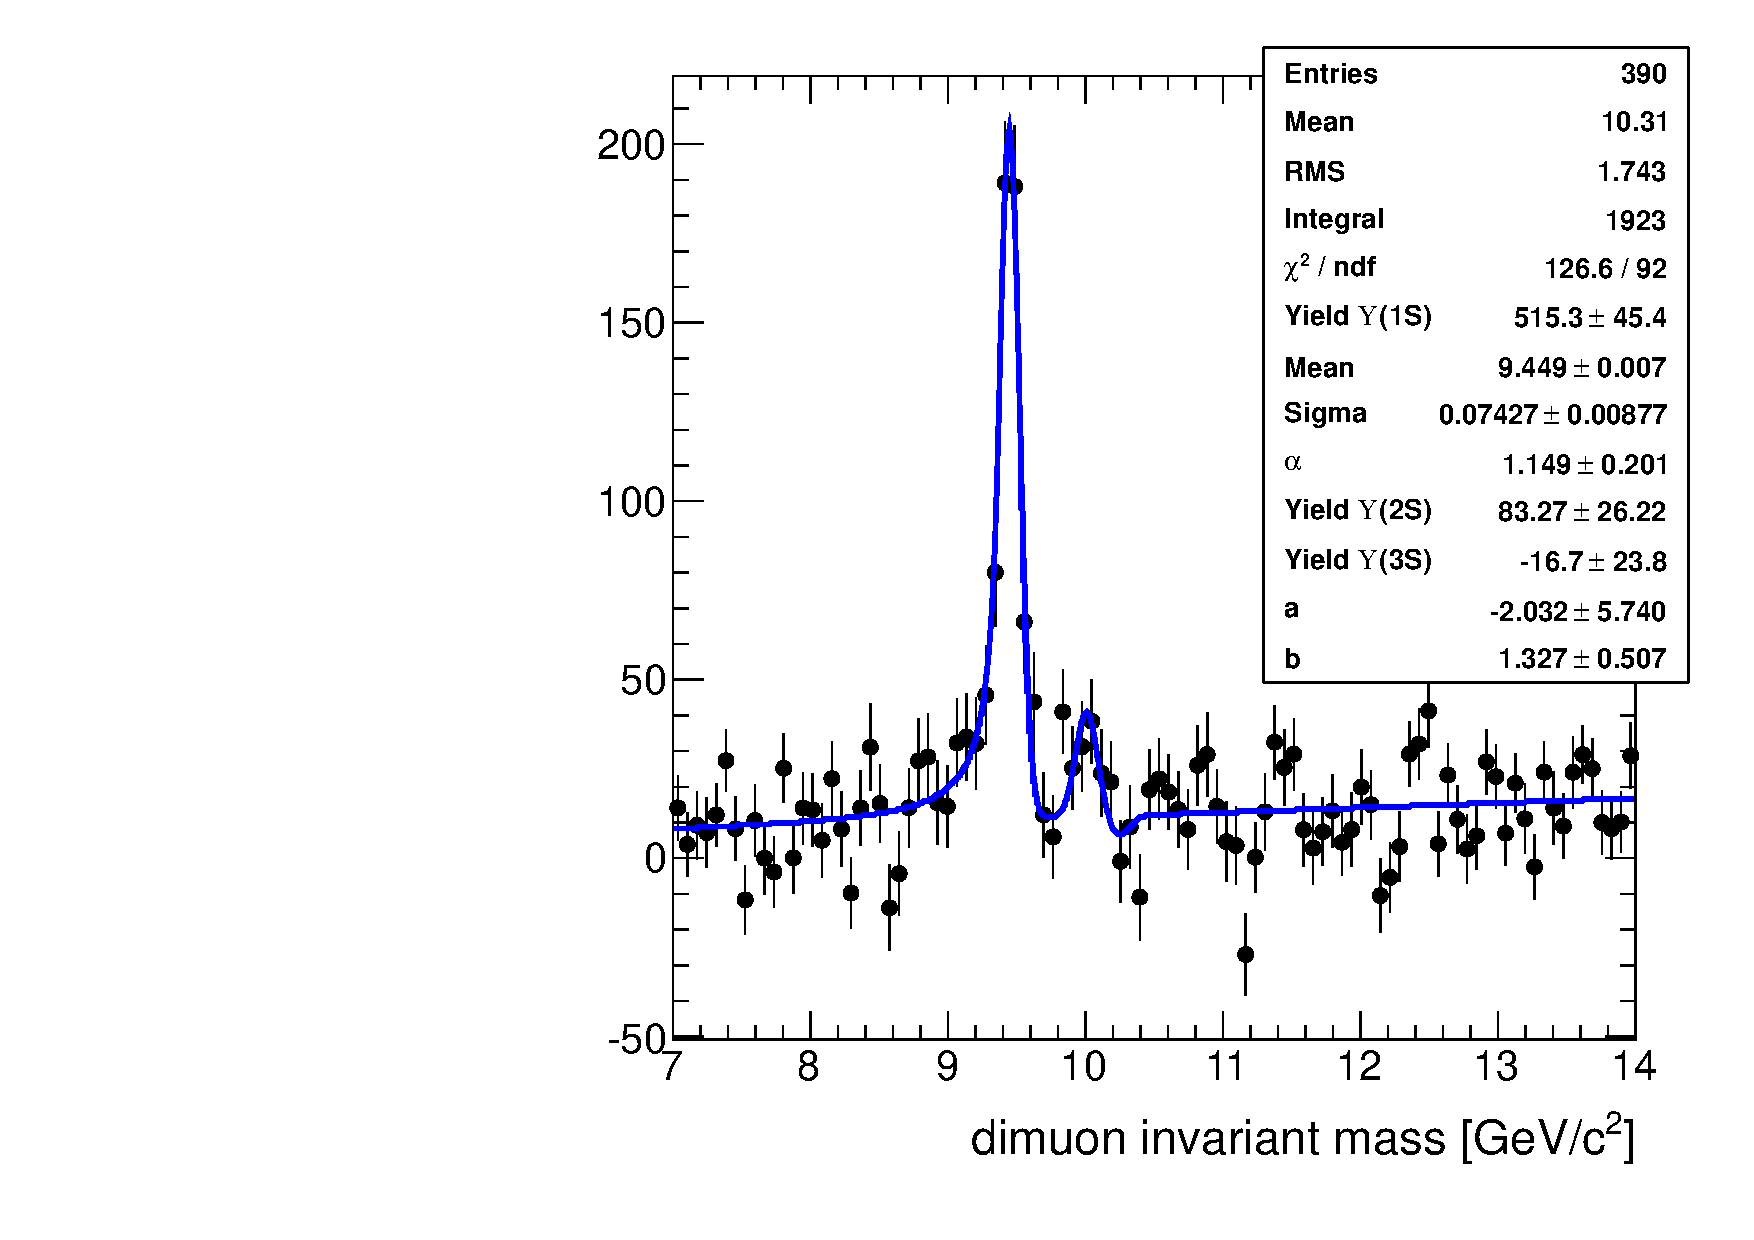
\includegraphics[angle=0,width=0.3\textwidth]{figures/fitting/fit_subtract_1stOrder_fixn_100bin.pdf}}
    \subfigure[bins:70]{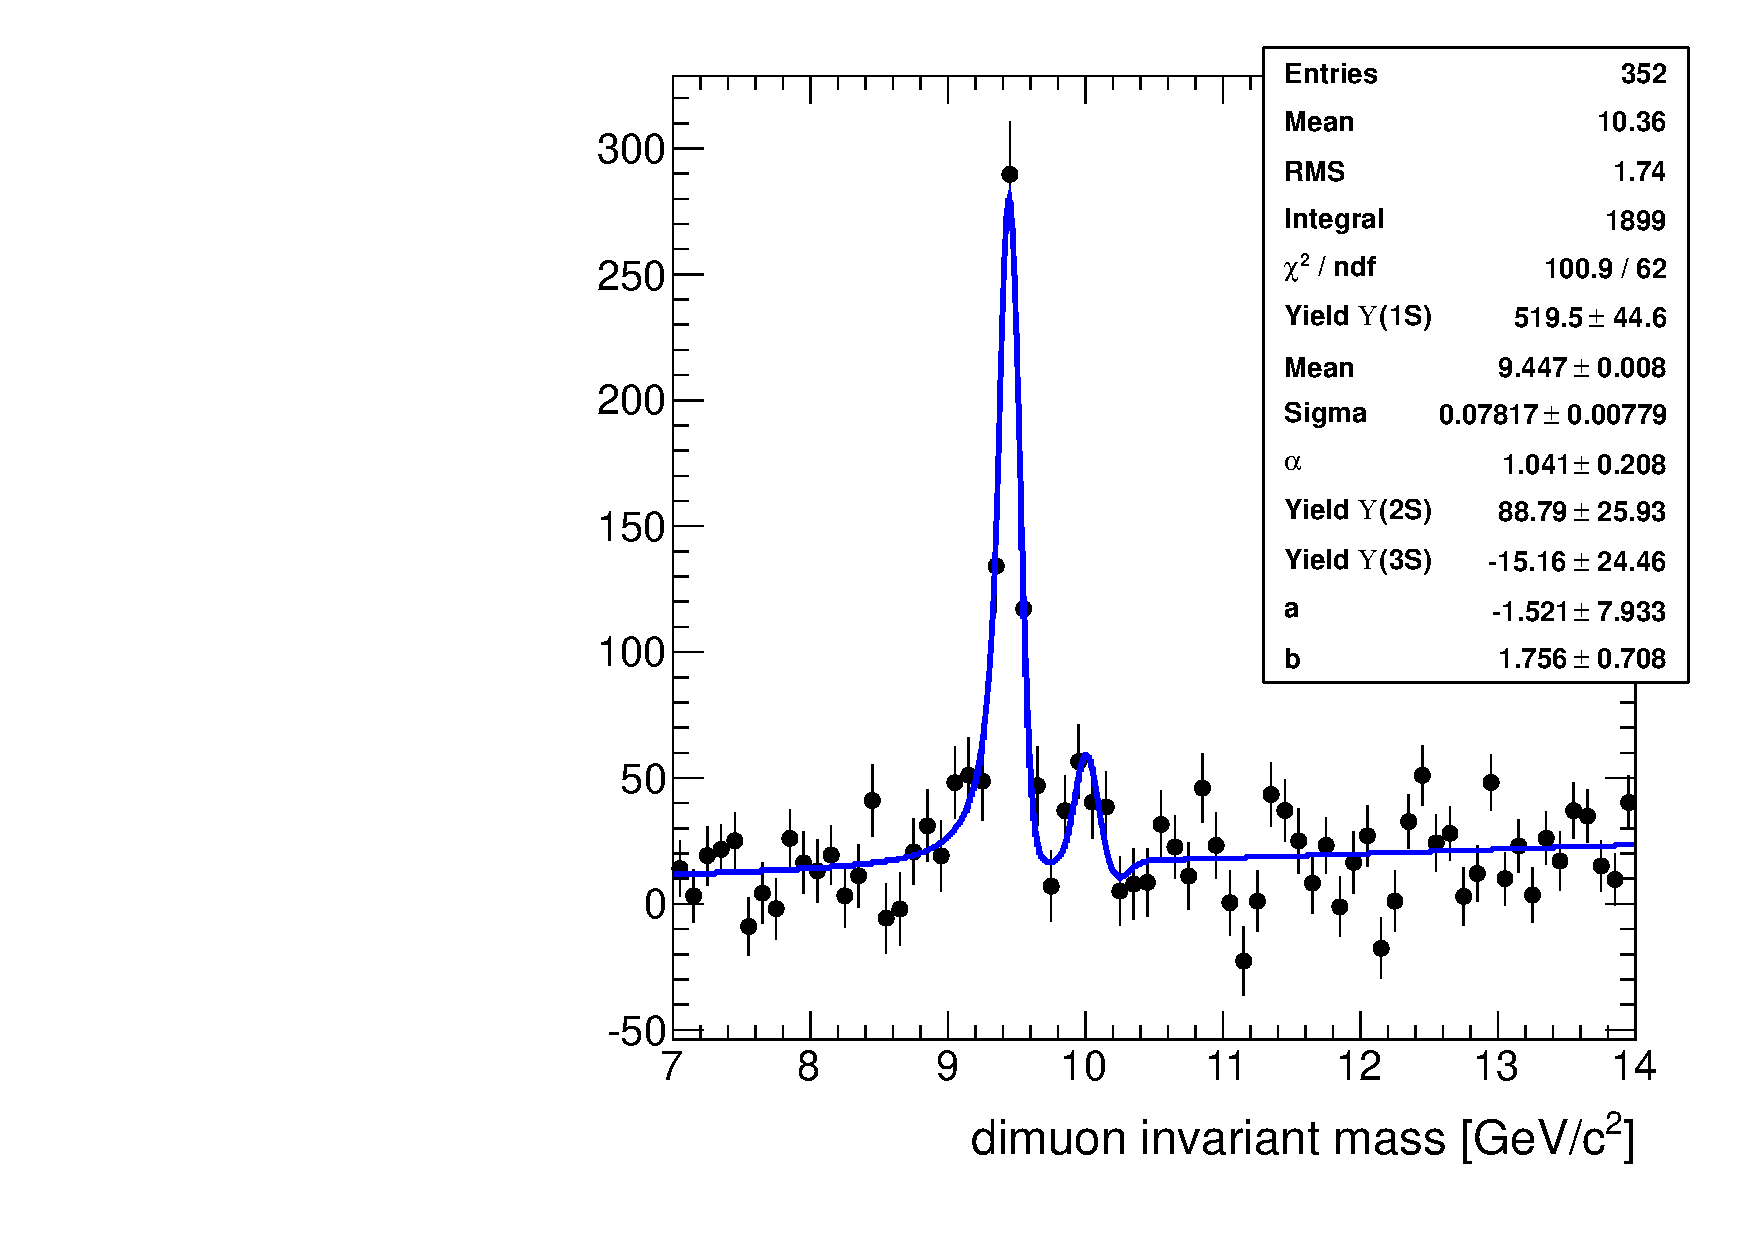
\includegraphics[angle=0,width=0.3\textwidth]{figures/fitting/fit_subtract_1stOrder_fixn_70bin.pdf}}
    \subfigure[bins:50]{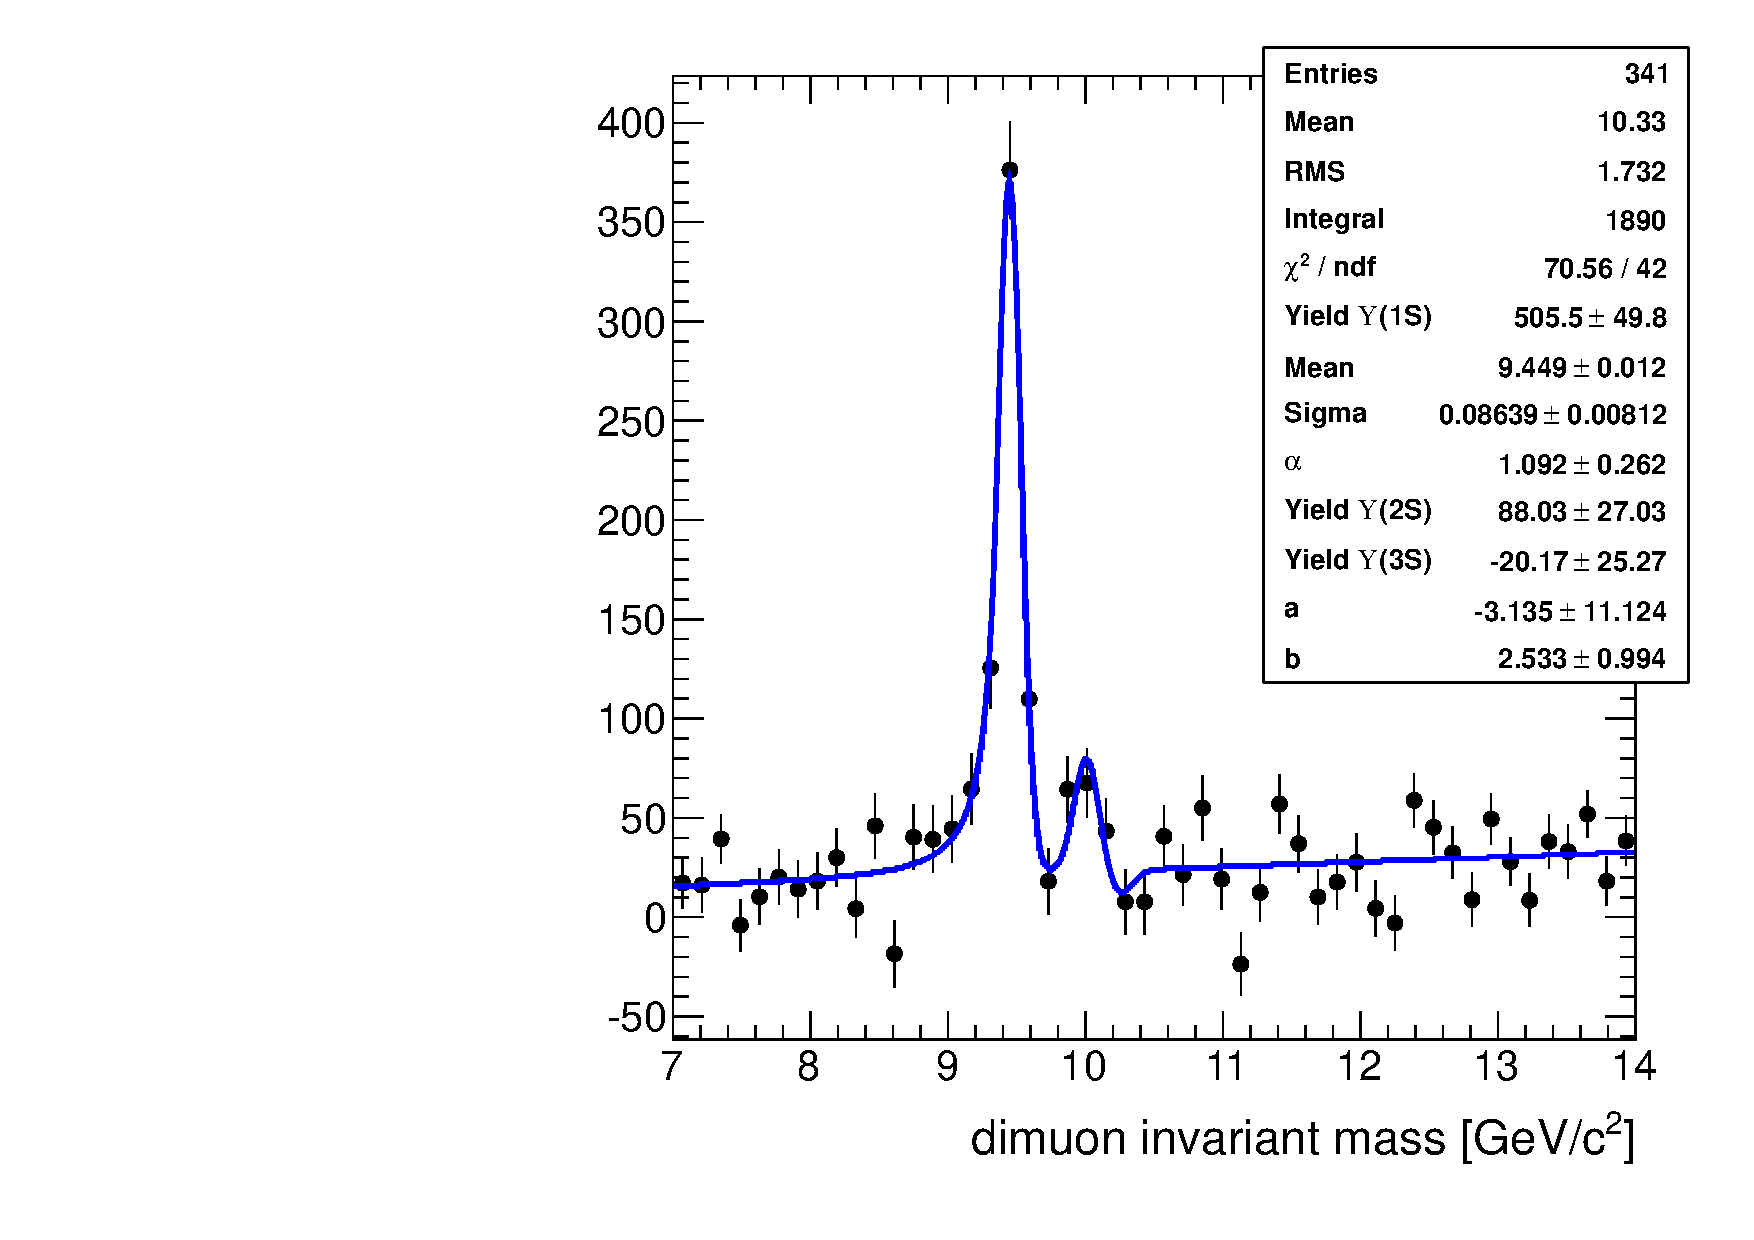
\includegraphics[angle=0,width=0.3\textwidth]{figures/fitting/fit_subtract_1stOrder_fixn_50bin.pdf}}
  \caption{FSR parameter estimation from like-sign subtracted data.}
  \label{fig:fsr_data_bins}
  \end{center}
\end{figure}



Table~\ref{tab:fsr} summarizes the CB tail parameter estimations achieved from simulation and data. 
%
It illustrates the level of variations that may be attained. 
In the nominal configuration, the $\alpha$ CB parameter is determined from the fit to the data. 
%
\begin{table}[!h]
  \centering
  \caption{Final state radiation and resolution parameter values.}
  \begin{tabular}{c|c c c}
    \hline
    & $\alpha$ & $n$ (fixed) & $\sigma \; (\MeVcc)$ \\
    \hline
    Monte Carlo   & $1.67 $ & 2.3  & $90$ \\
    \pp 7 TeV data  & $1.4 \pm 0.1$ & 2.3  & $62 \pm 2$ \\
    like-sign subtracted \PbPb data & $1.0 \pm  0.3$ & 2.3 & $73 - 87$ \\ %TBD: needs to re-done withh corercted data!!
    \PbPb data (nominal fit) & $0.98 \pm 0.2 $ & 2.3  & $78.2 \pm 0.5$ \\
    \PbPb and \pp data (nominal simul. fit) & $1.12 \pm 0.13 $ & 2.3 & $79.4 \pm 0.4$\\
    \hline
  \end{tabular}
  \label{tab:fsr}
\end{table}
%https://espace.cern.ch/cms-heavyion/upsilon/fitting/fsr_pp_study.aspx
%https://espace.cern.ch/cms-heavyion/upsilon/fitting/likesign_181912-182609.aspx
%https://espace.cern.ch/cms-heavyion/upsilon/fitting/RadiationTailFromMC.aspx

%\FloatBarrier

\subsection{Background model studies}
\label{sec:bgmodel}

%Previosuly~\cite{prl}, the background has been described by a second-order polynominal in the mass-fitting range $7-14\GeVcc$. 
%In view of the increased statistics, a more detailed treatment is now pursued, as documented in the following sections. 

We explore alternative estimations and parameterizations of the background, with respect to the second order polynomial model used in~\cite{CMS_AN_2010-140, CMS_AN_2011_062}.  

\subsubsection{Like-sign dimuon spectrum}
\label{sec:like-sign}

Here we carry out fits to the upsilon data, by constraining the background model utilizing information from the like-sign dimuon spectrum. 
The like-sign dimuon combinations contain no signal component, and provide a useful handle to estimate the combinatorial background shape in the mass region under the signal peaks. 
The like-sign spectrum is not expected to match \emph{exactly}, in shape and normalization, the combinatorial opposite-side spectrum: 
different, small contributions may arise from Drell-Yan and open flavor sources. This residual component is expected to be smooth and non-peaking, and is accommodated by allowing an extra polynomial component in the fit the (oppositely charged dimuon) data. 

The like-sign dimuon mass distribution is employed to define a PDF component, in the following two ways: 
\begin{itemize} 
\item {\bf{Like-sign dataset smoothing.}} 
We use the RooFit implementation via the class RooKeysPdf~\cite{rookeyspdf}, which implements a one-dimensional kernel estimation PDF which models (smoothens) the distribution %of an arbitrary input dataset 
as a superposition of Gaussian kernels, one for each data point, each contributing 1/N to the total integral of the PDF.  
%\emph{(add reference: Cranmer KS, Kernel Estimation in High-Energy Physics. Computer Physics Communications 136:198-207,2001 - e-Print Archive: hep ex/0011057)} 

\item {\bf{Like-sign parameterized fit.}} 
We fit the like-sign distribution utilizing an $\text{Erf} \times \text{Exp}$ model. 
The high-mass spectrum is well described by an exponential,  
%We motivate the exponential to account 
describing random track combinations. 
To describe the acceptance turn-on shape induced by the single muon kinematic threshold, 
 %below the $\PgU$ peak ????
the exponential is multiplied by an error function. 
%an error-function is multiplied to the .
 %like-sign combinations at higher mass. 
%For $\pt>3.5 \GeVc$ the parameters are $m0shift$ $6.910 \pm 0.073 \GeVcc$ and $width$ $1.18 \pm 0.21 \GeVcc$. 
Tested variations of the turn-on function parameters gave negligible deviations of the extracted yields. 
\end{itemize} 

The shape of the like-sign distribution matches well that of the mass sidebands in the opposite-sign sample. 
The fit to the opposite-sign signal sample is performed employing a linear combination of the like-sign extracted PDF,  along with an extra polynomial component. The latter is included in order to allow for potential discrepancies that might arise between the like-sign and opposite-sign mass spectra.
The fit results are displayed in~\fig{fig:massfits_likesign} 
%(and in~\fig{fig:massfits_likesign_35} fot the 3.5 \GeVc cut instead of the nominal 4.0), 
and demonstrate a good description of the data. 


\begin{figure}[hbtp]
  \begin{center}
    \subfigure[$\pt^\mu>3.5\GeVc$, rookeyspdf, $70 \mu b^{-1}$]{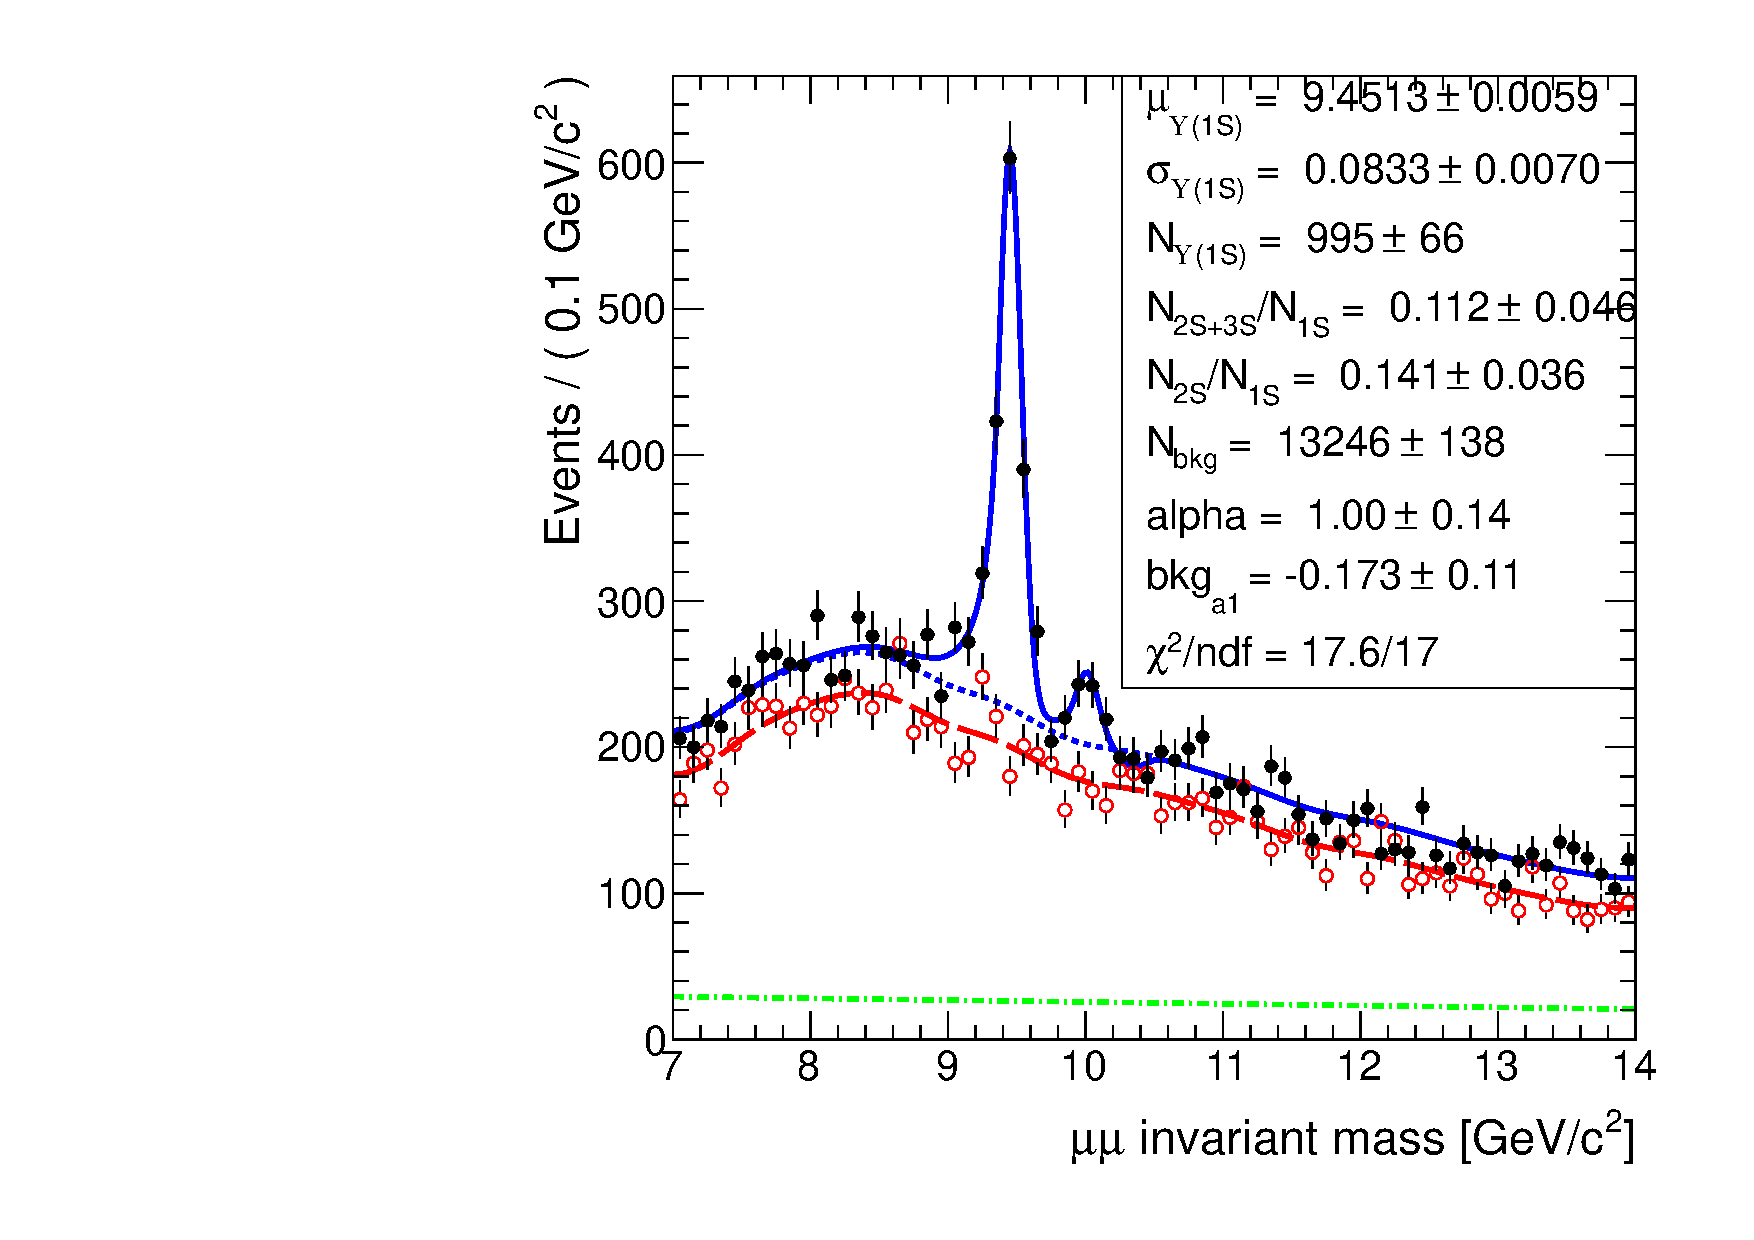
\includegraphics[angle=0,width=0.5\textwidth]{figures/fitting/masspeak_Hi_paramOn_MuonPT35_liner}}
    \subfigure[$\pt^\mu>4.0\GeVc$, rookeyspdf, $150 \mu b^{-1}$]{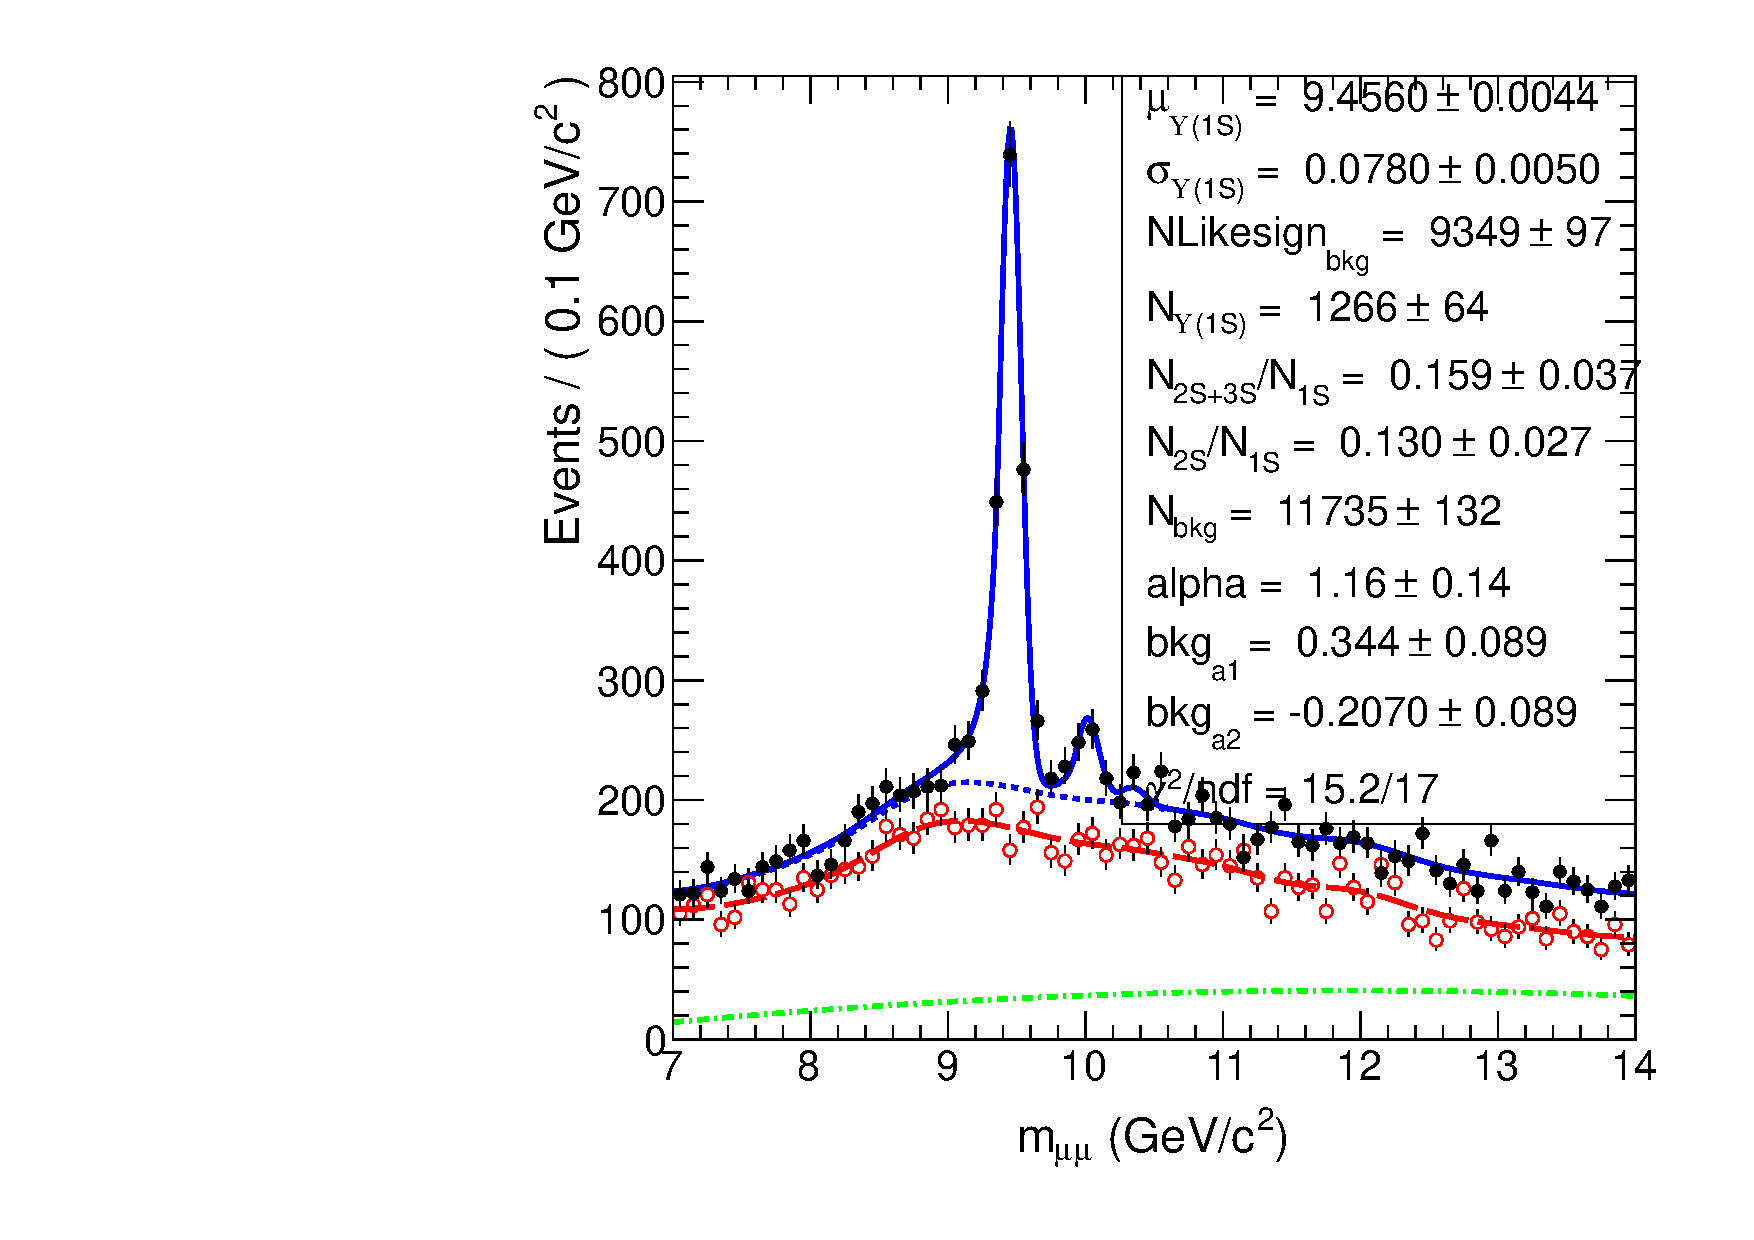
\includegraphics[angle=0,width=0.5\textwidth]{figures/fitting/masspeak_Hi_paramOn_liner}}\\
    \subfigure[$\pt^\mu>3.5\GeVc$,    exp*erf, $70 \mu b^{-1}$]{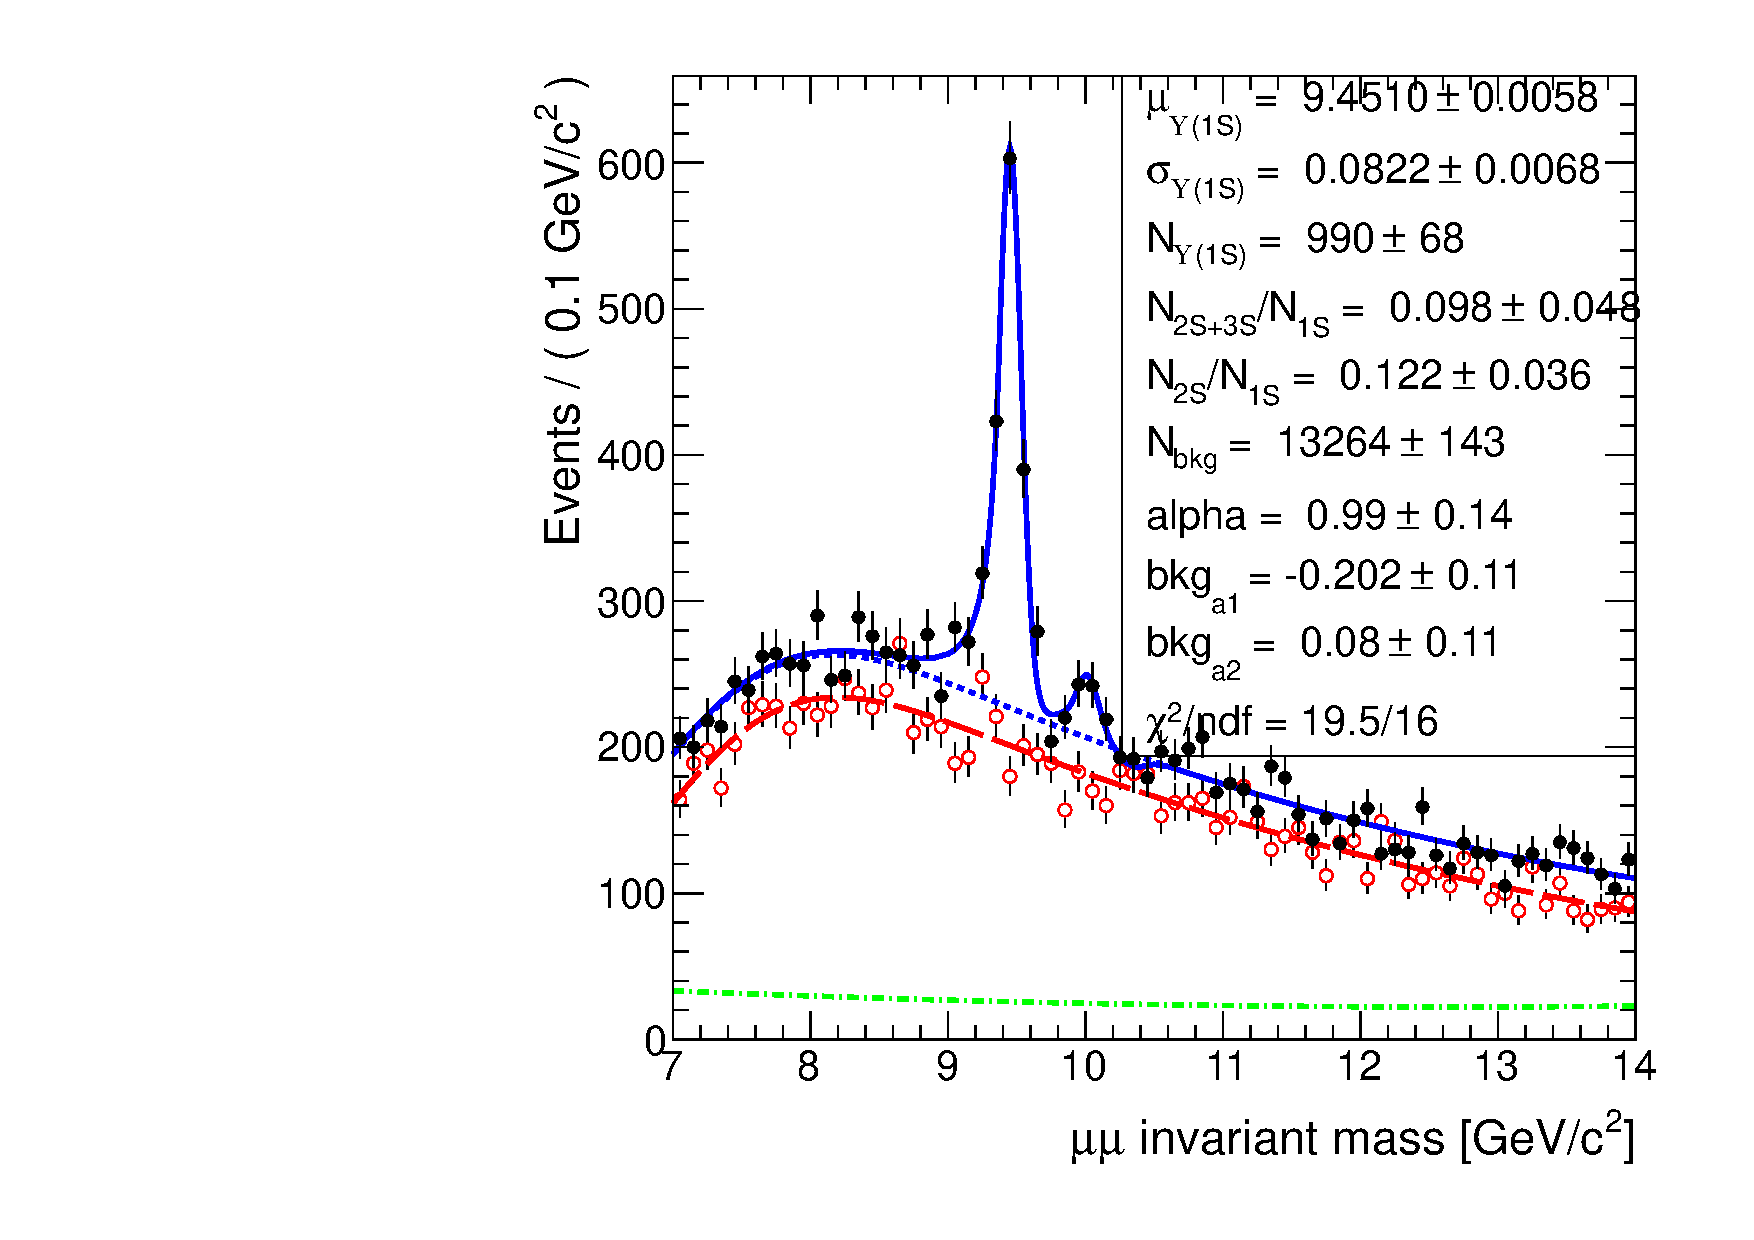
\includegraphics[angle=0,width=0.5\textwidth]{figures/fitting/masspeak_Hi_paramOn_ErrFunc_MuonPT35}}
    \subfigure[$\pt^\mu>4.0\GeVc$,    exp*erf, $150 \mu b^{-1}$]{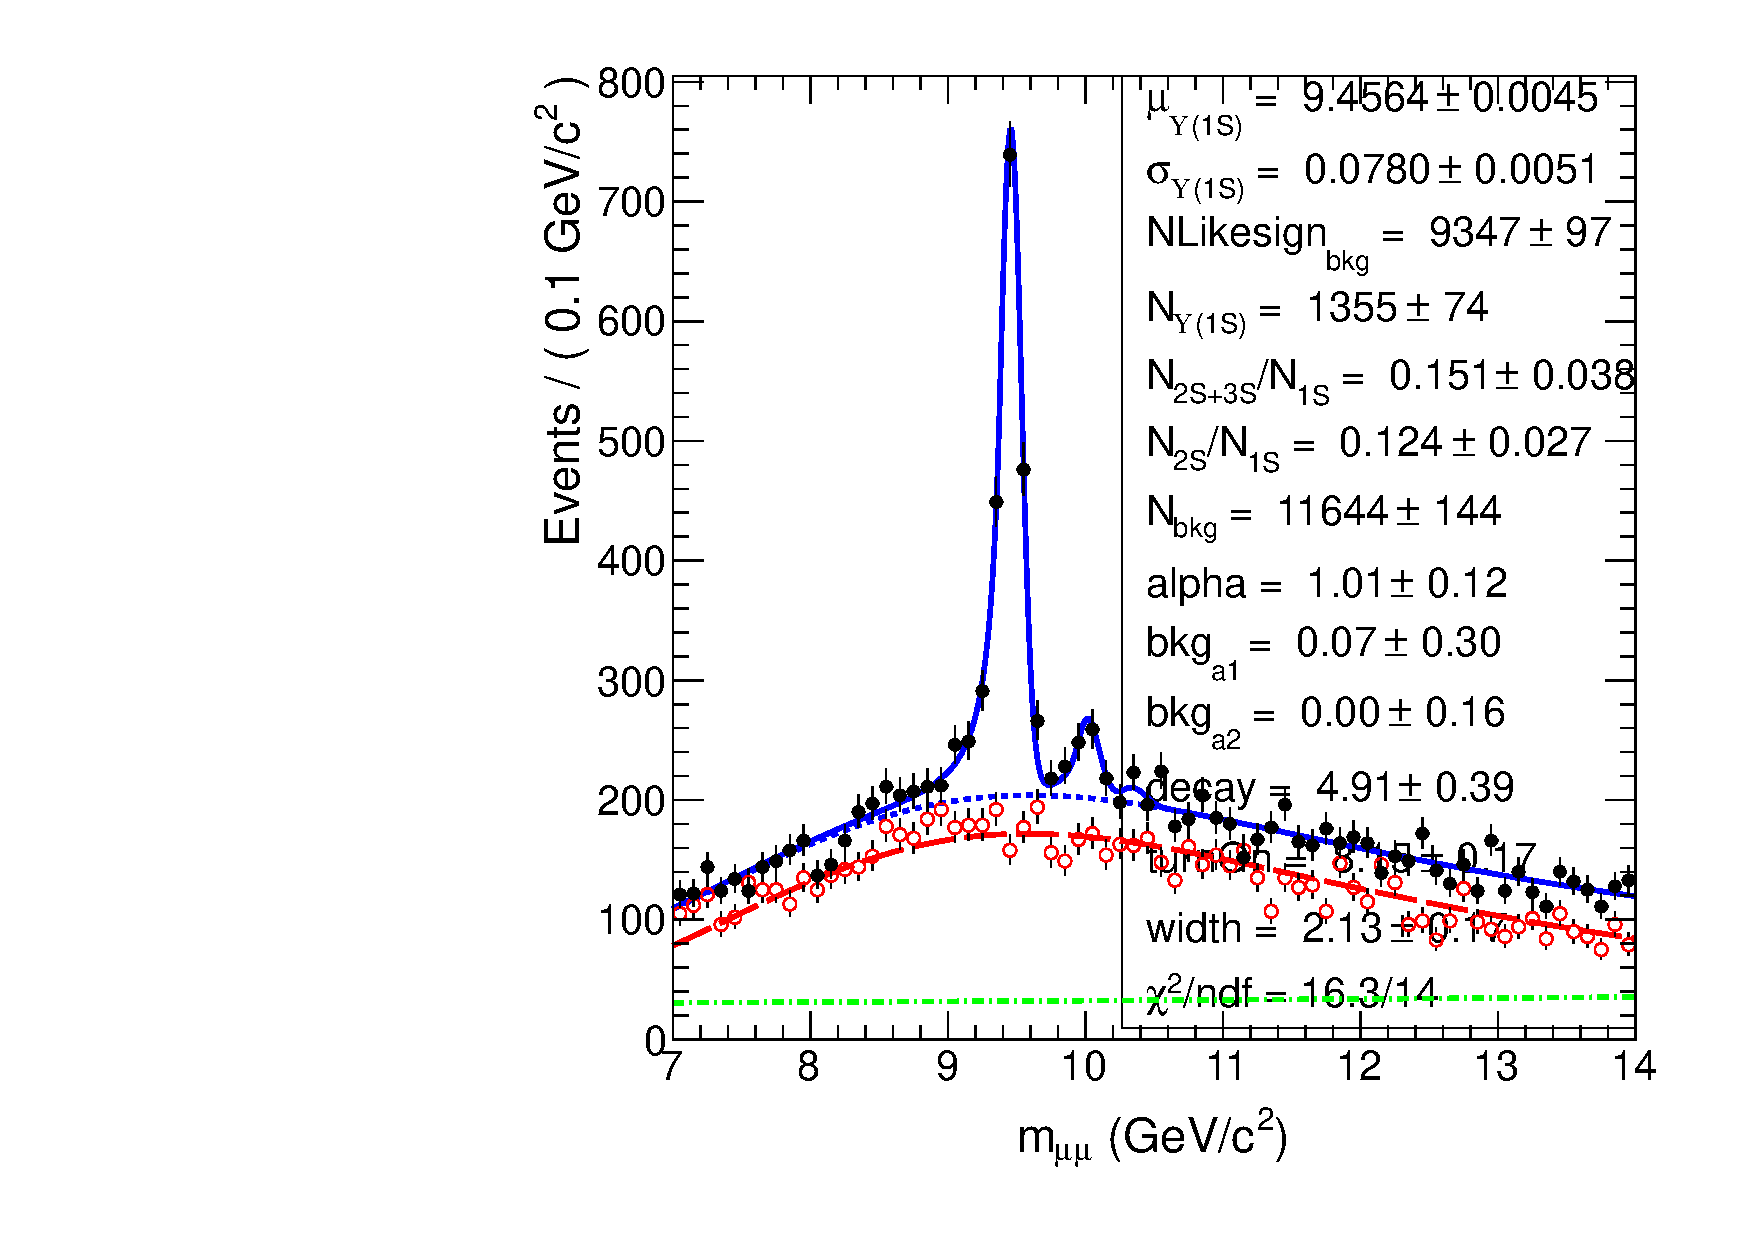
\includegraphics[angle=0,width=0.5\textwidth]{figures/fitting/masspeak_Hi_paramOn_ErrFunc}}
    \caption{Mass fits, with background constrained from like-sign dimuon spectrum.}
    \label{fig:massfits_likesign}
  \end{center}
\end{figure}

%\begin{figure}[hbtp]
%  \begin{center}
%    %\subfigure[]
%    {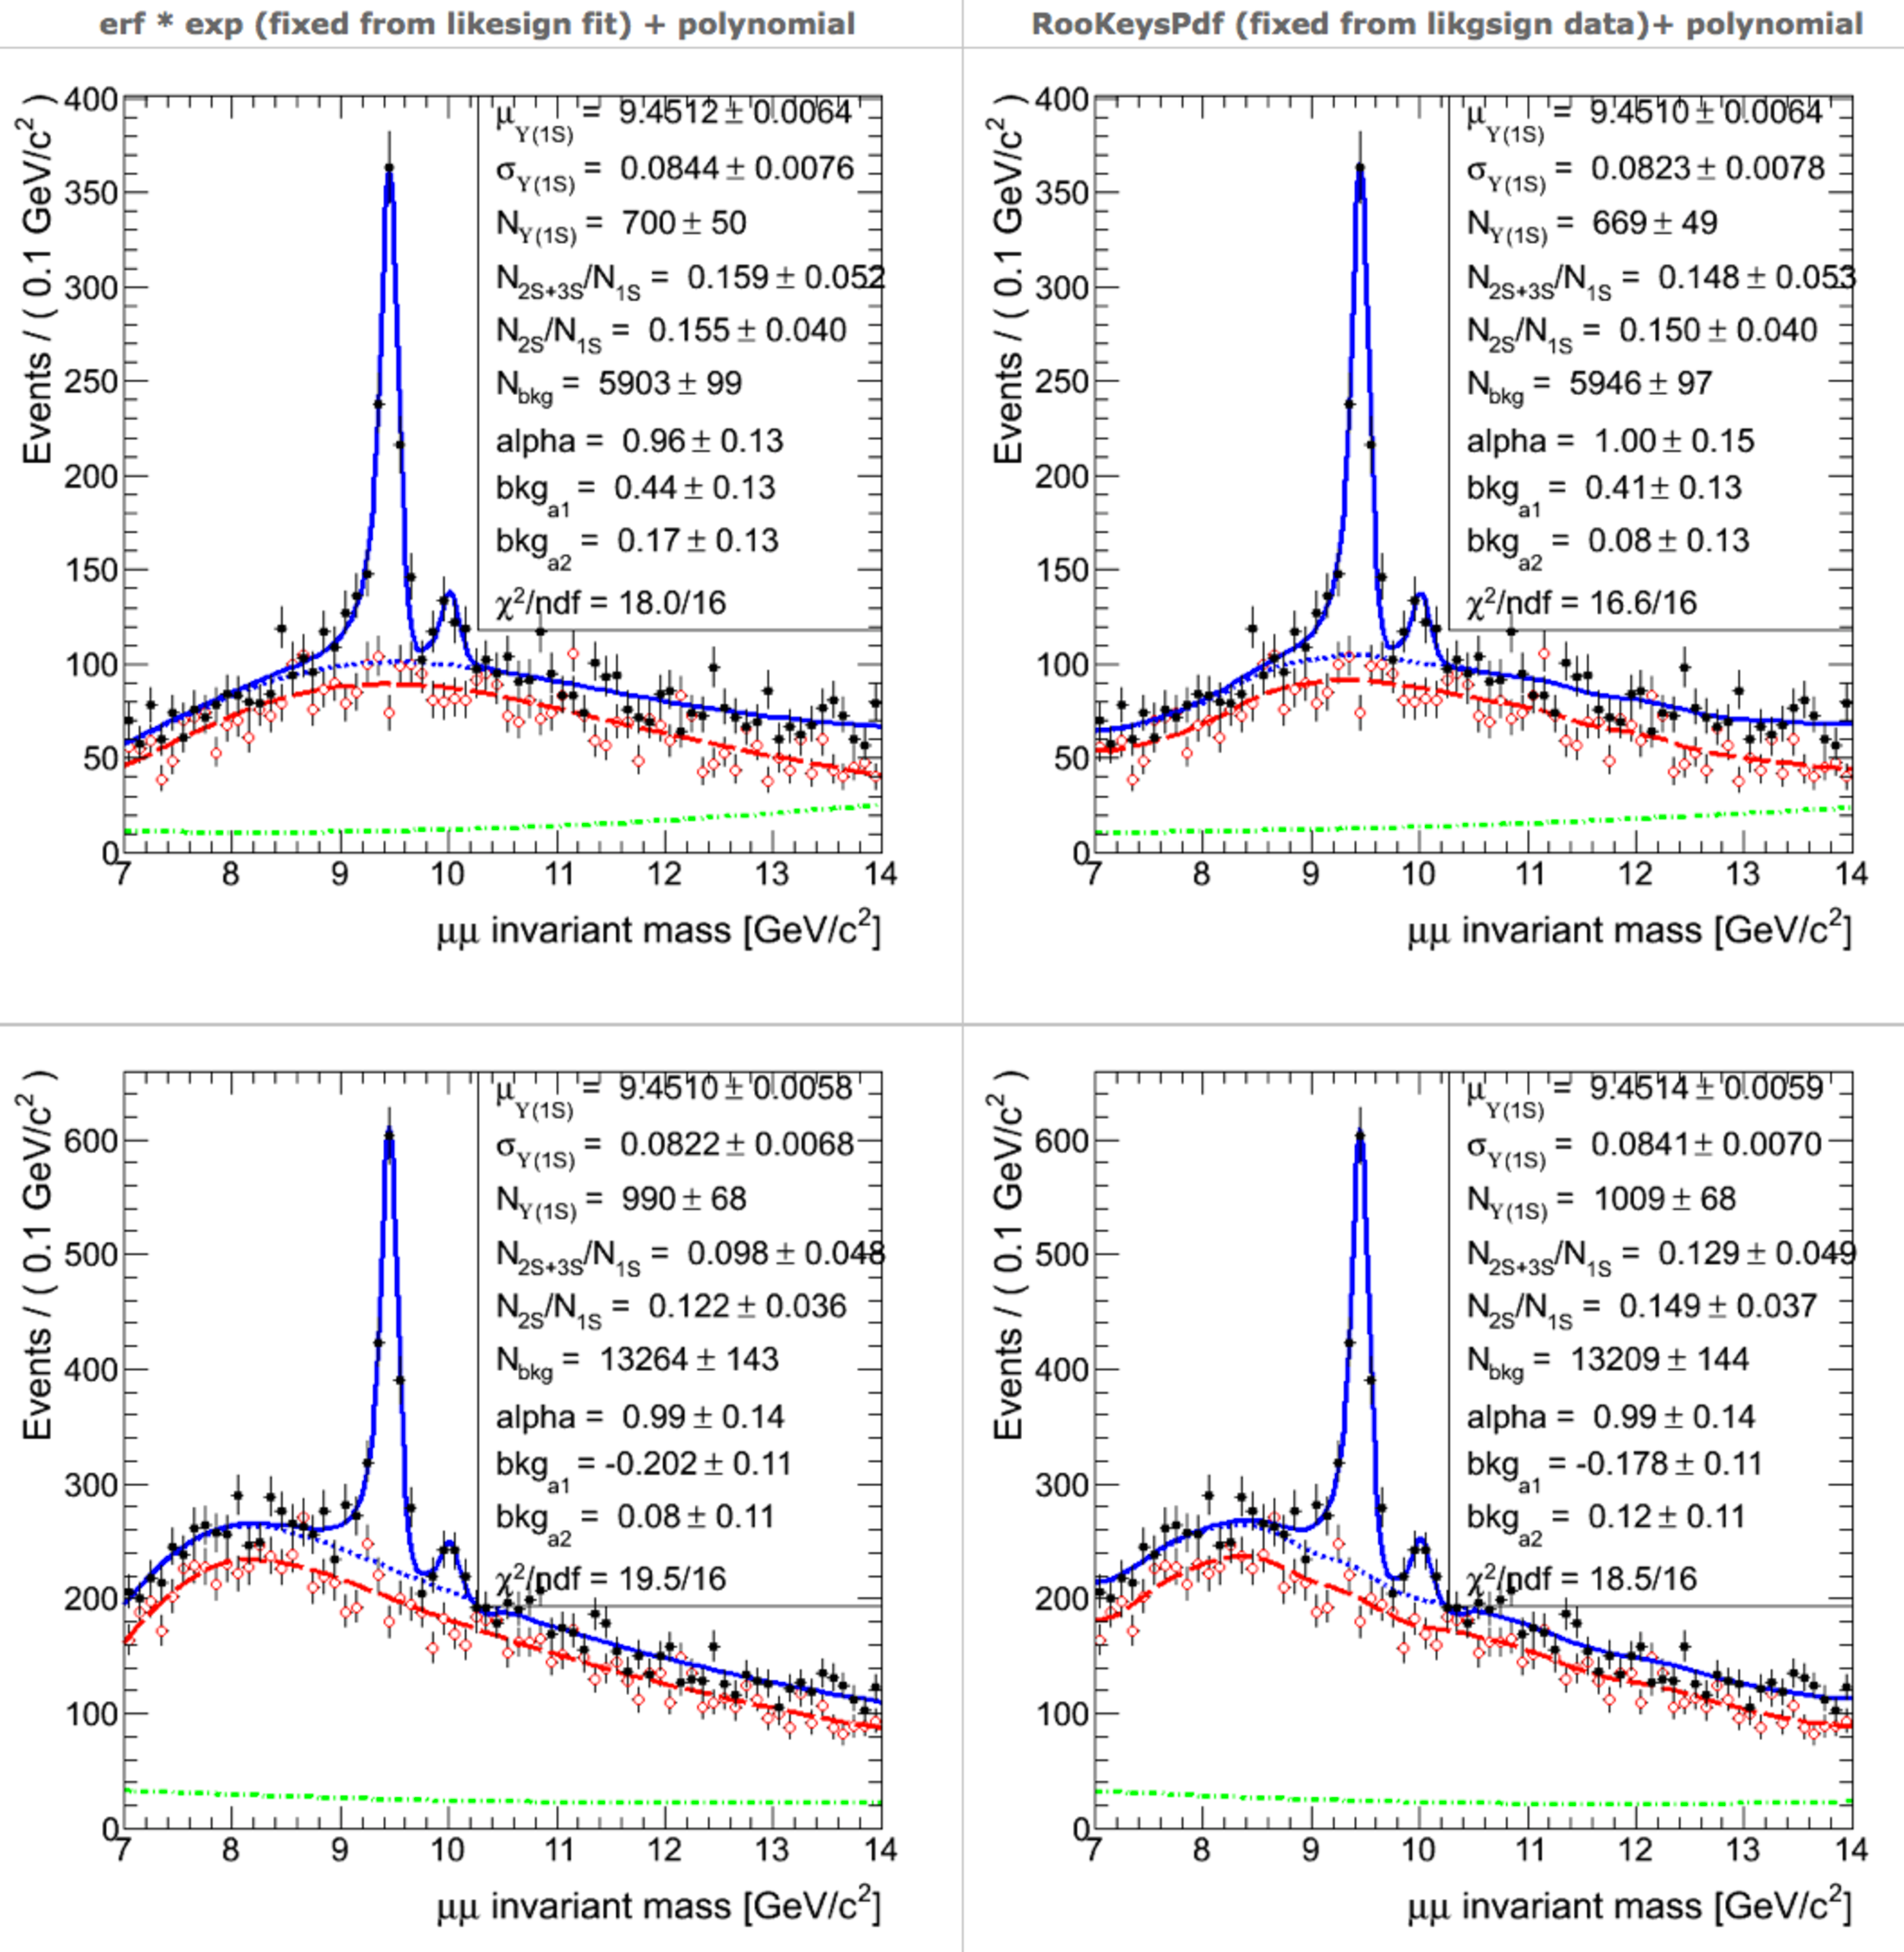
\includegraphics[angle=0,width=1\textwidth]{figures/fitting/massfits_likesign_option2}}
%    \caption{Mass fits, with background constrained from like-sign dimuon spectrum.}
%    \label{fig:massfits_likesign}
%  \end{center}
%\end{figure}



\subsubsection{Track-rotation method}
\label{sec:track-rotsation}

We explore an independent method to estimate the combinatorial background. 
This is normally referred to as ``track-rotation method'' and consists of the following steps:
(i) all like-sign muon pairs (or the unlike-sign muon pairs) in the event are formed, 
(ii) for each pair, one of the muons is randomly selected, and 
(iii) its $\phi$ coordinate is rotated by $\pi$. 
In this way we obtain an uncorrelated sample of tracks, extracted directly from the data and thus matching the data kinematics, 
from which the combinatorial mass distribution can be estimated. 

Having extracted the combinatorial background PDF, the same fitting strategy as described in Sec.~\ref{sec:like-sign} for the like-sign case is employed when fitting the oppositely charged dimuon data. The track rotation PDF is normalized to like-sign yield. 
The results are shown in~\fig{fig:track_rotation} for like-sign, in~\fig{fig:track_rotation_OS} for unlikesign. They display a good description of the data.
A comparison of like-sign pairs shape, track rotation pairs shape, and unlike-sign pairs shape is shown in~\fig{fig:compareBkgd}.

\begin{figure}[hbtp]
  \begin{center}
	\subfigure[erf*exp + pol.2]{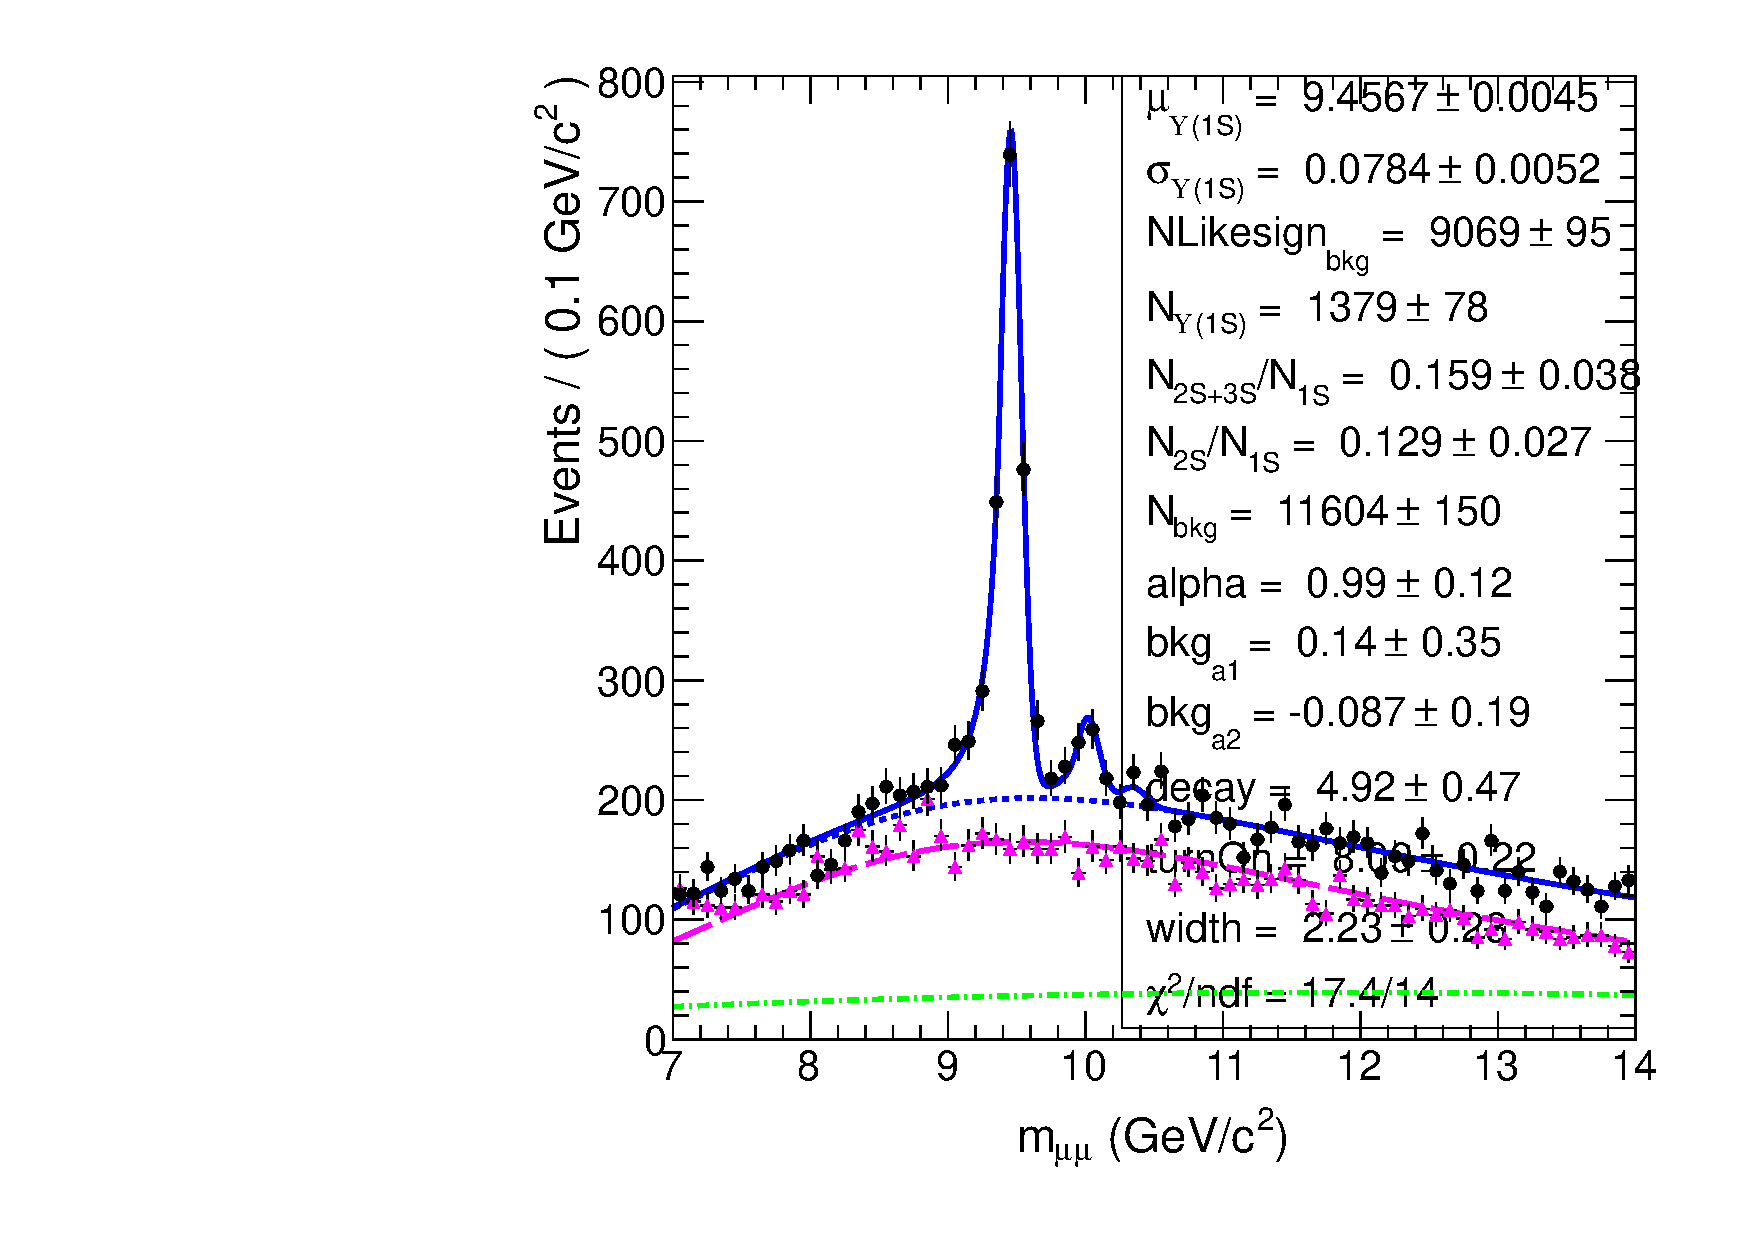
\includegraphics[angle=0,width=0.5\textwidth]{figures/fulldataset/masspeak_hi_TRerf.pdf}}
    \subfigure[keysPdf + pol.2]{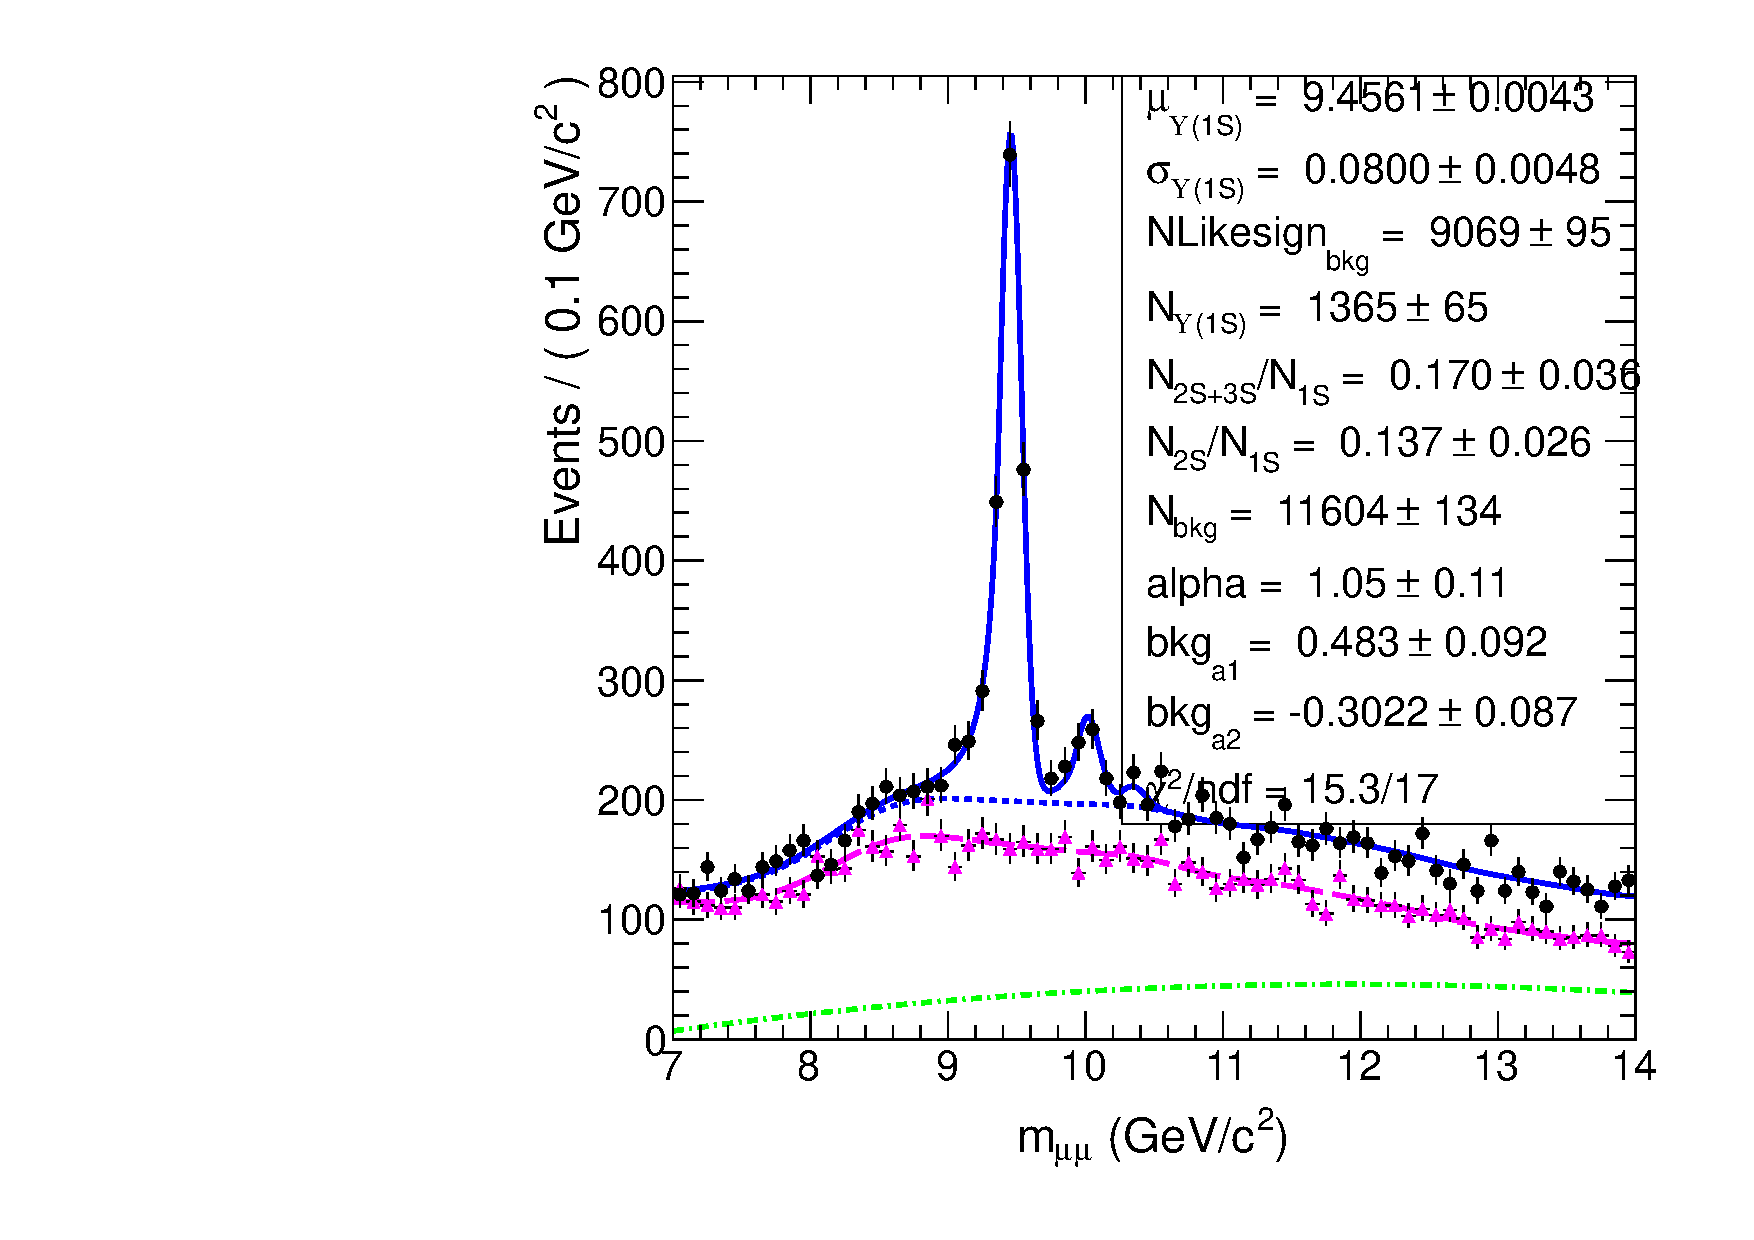
\includegraphics[angle=0,width=0.5\textwidth]{figures/fulldataset/masspeak_hi_TRkeys.pdf}}
    \caption{Mass fit, with background constrained from the track-rotated like-sign dimuon spectrum shown in magenta ($\pt^\mu>4.0\GeVc$, $150 \mu b^{-1}$).}
    \label{fig:track_rotation}
  \end{center}
\end{figure}

\begin{figure}[hbtp]
  \begin{center}
    \subfigure[erf*exp + pol.2]{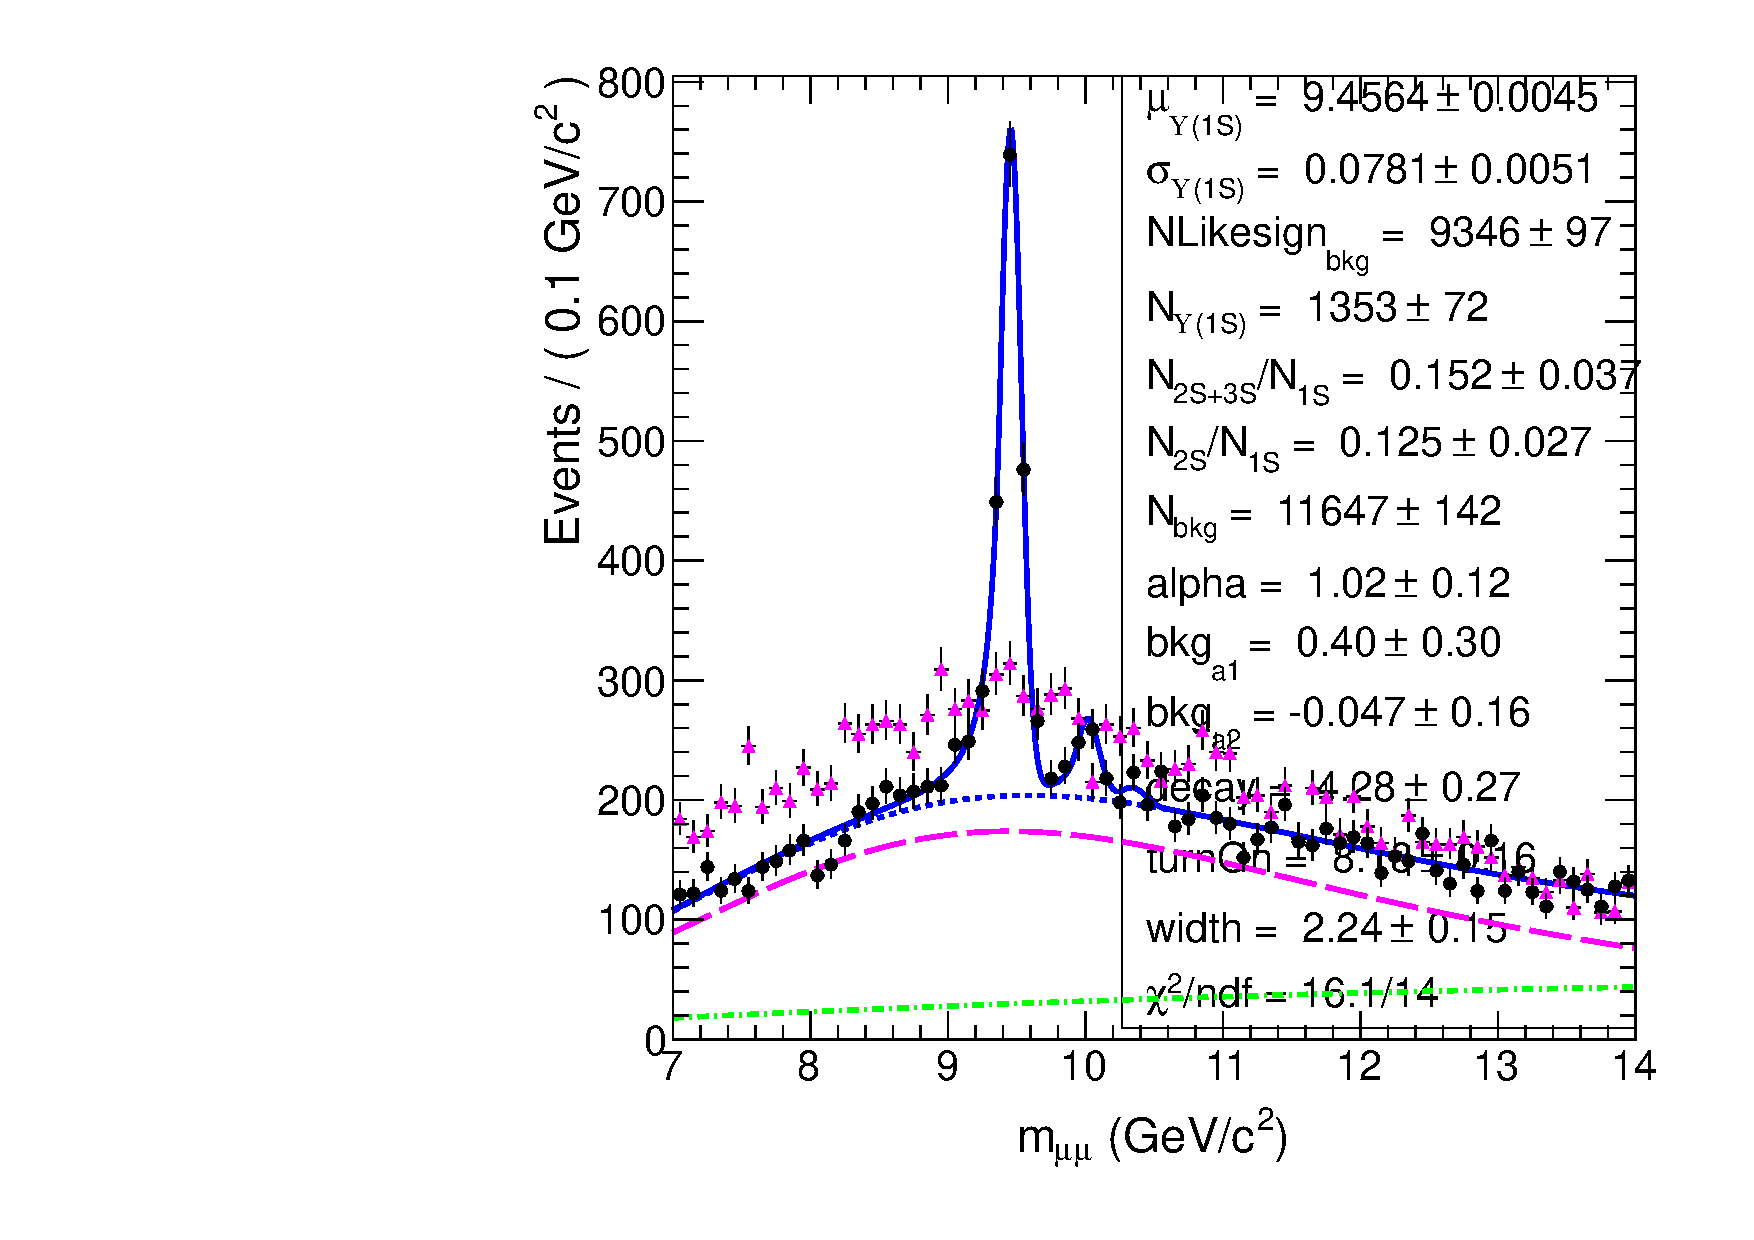
\includegraphics[angle=0,width=0.5\textwidth]{figures/fulldataset/masspeak_Hi_paramOn_OS_trkRot.pdf}}
    \subfigure[keysPdf + pol.2]{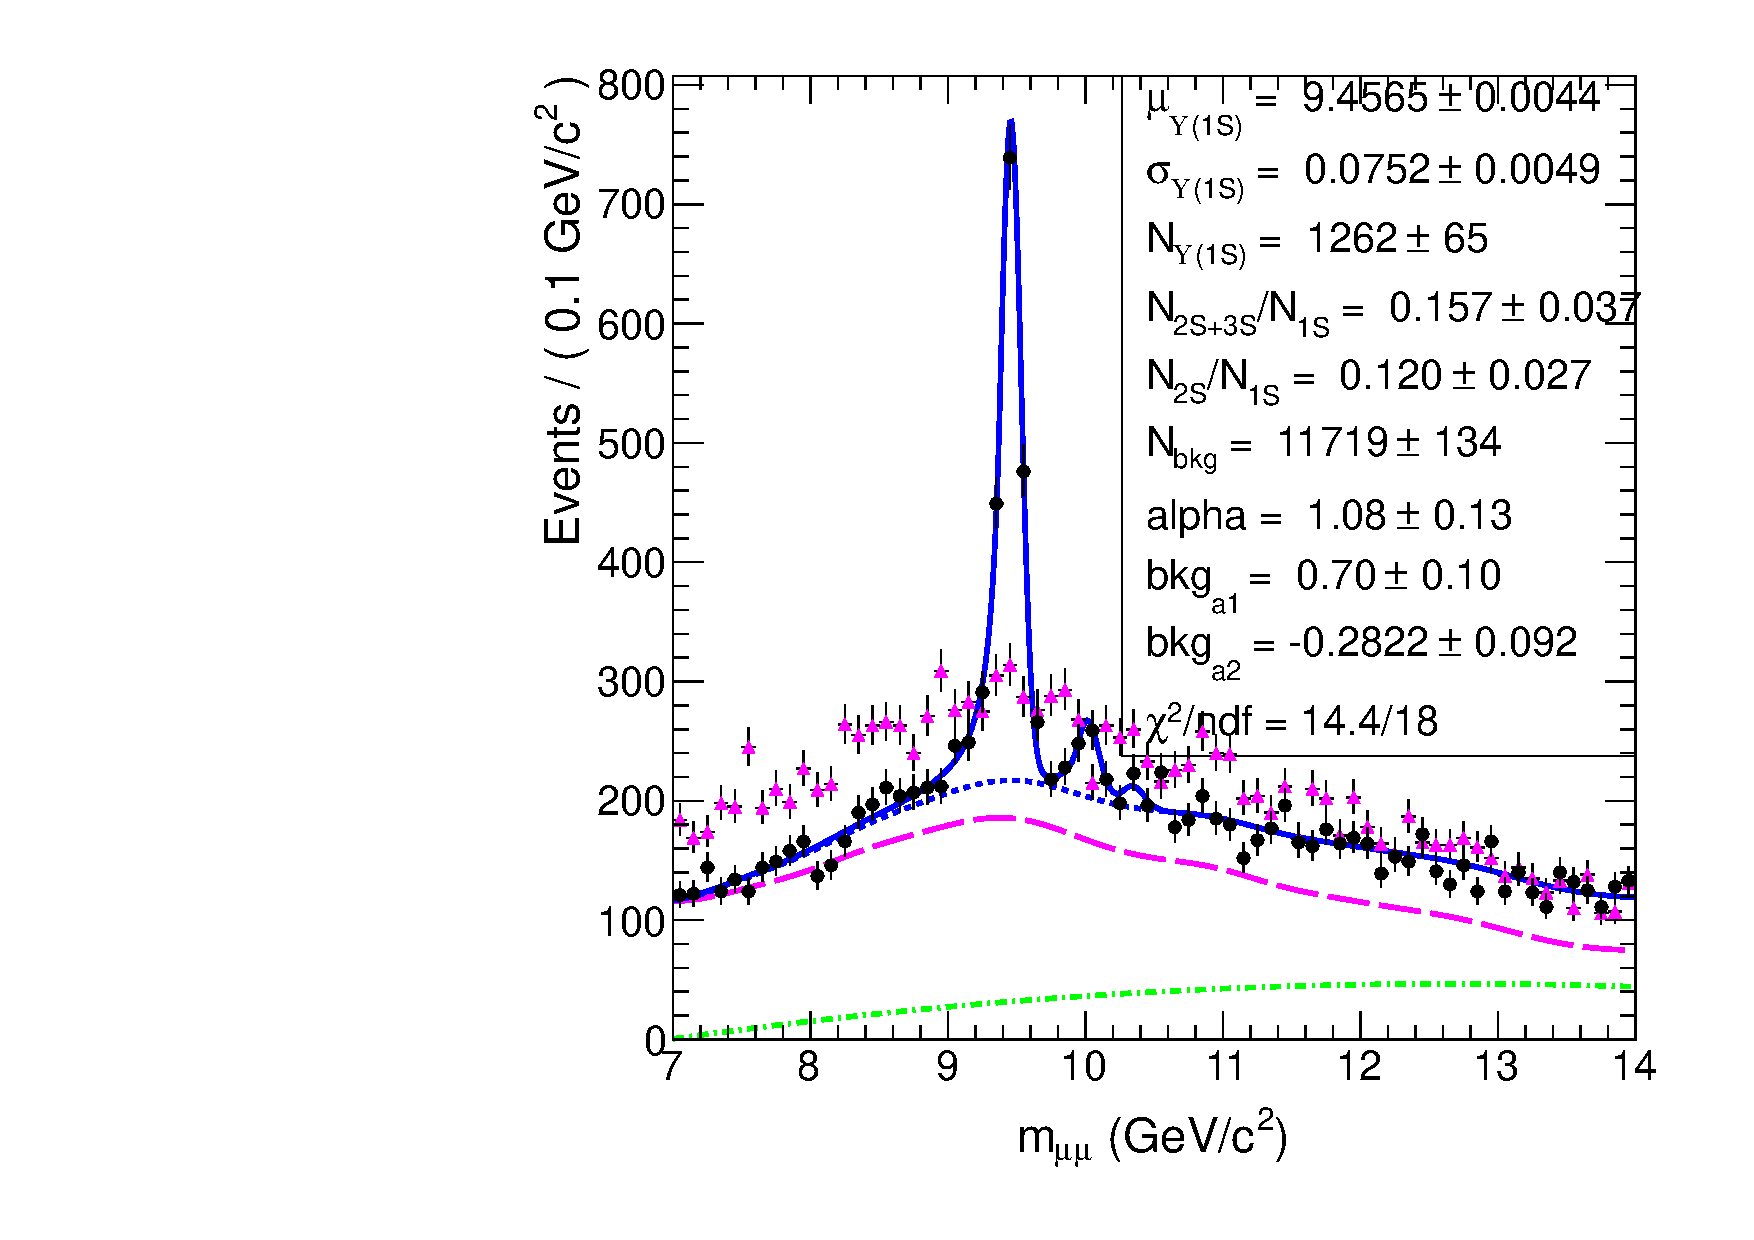
\includegraphics[angle=0,width=0.5\textwidth]{figures/fulldataset/masspeak_Hi_keysPdf_OS_trkRot.pdf}}
    \caption{Mass fit, with background constrained from the track-rotated unlike-sign dimuon spectrum shown in magenta points. The magenta curve is normalized to like-sign pairs yield.}
    \label{fig:track_rotation_OS}
  \end{center}
\end{figure}

\begin{figure}[h!]
 \begin{center}
    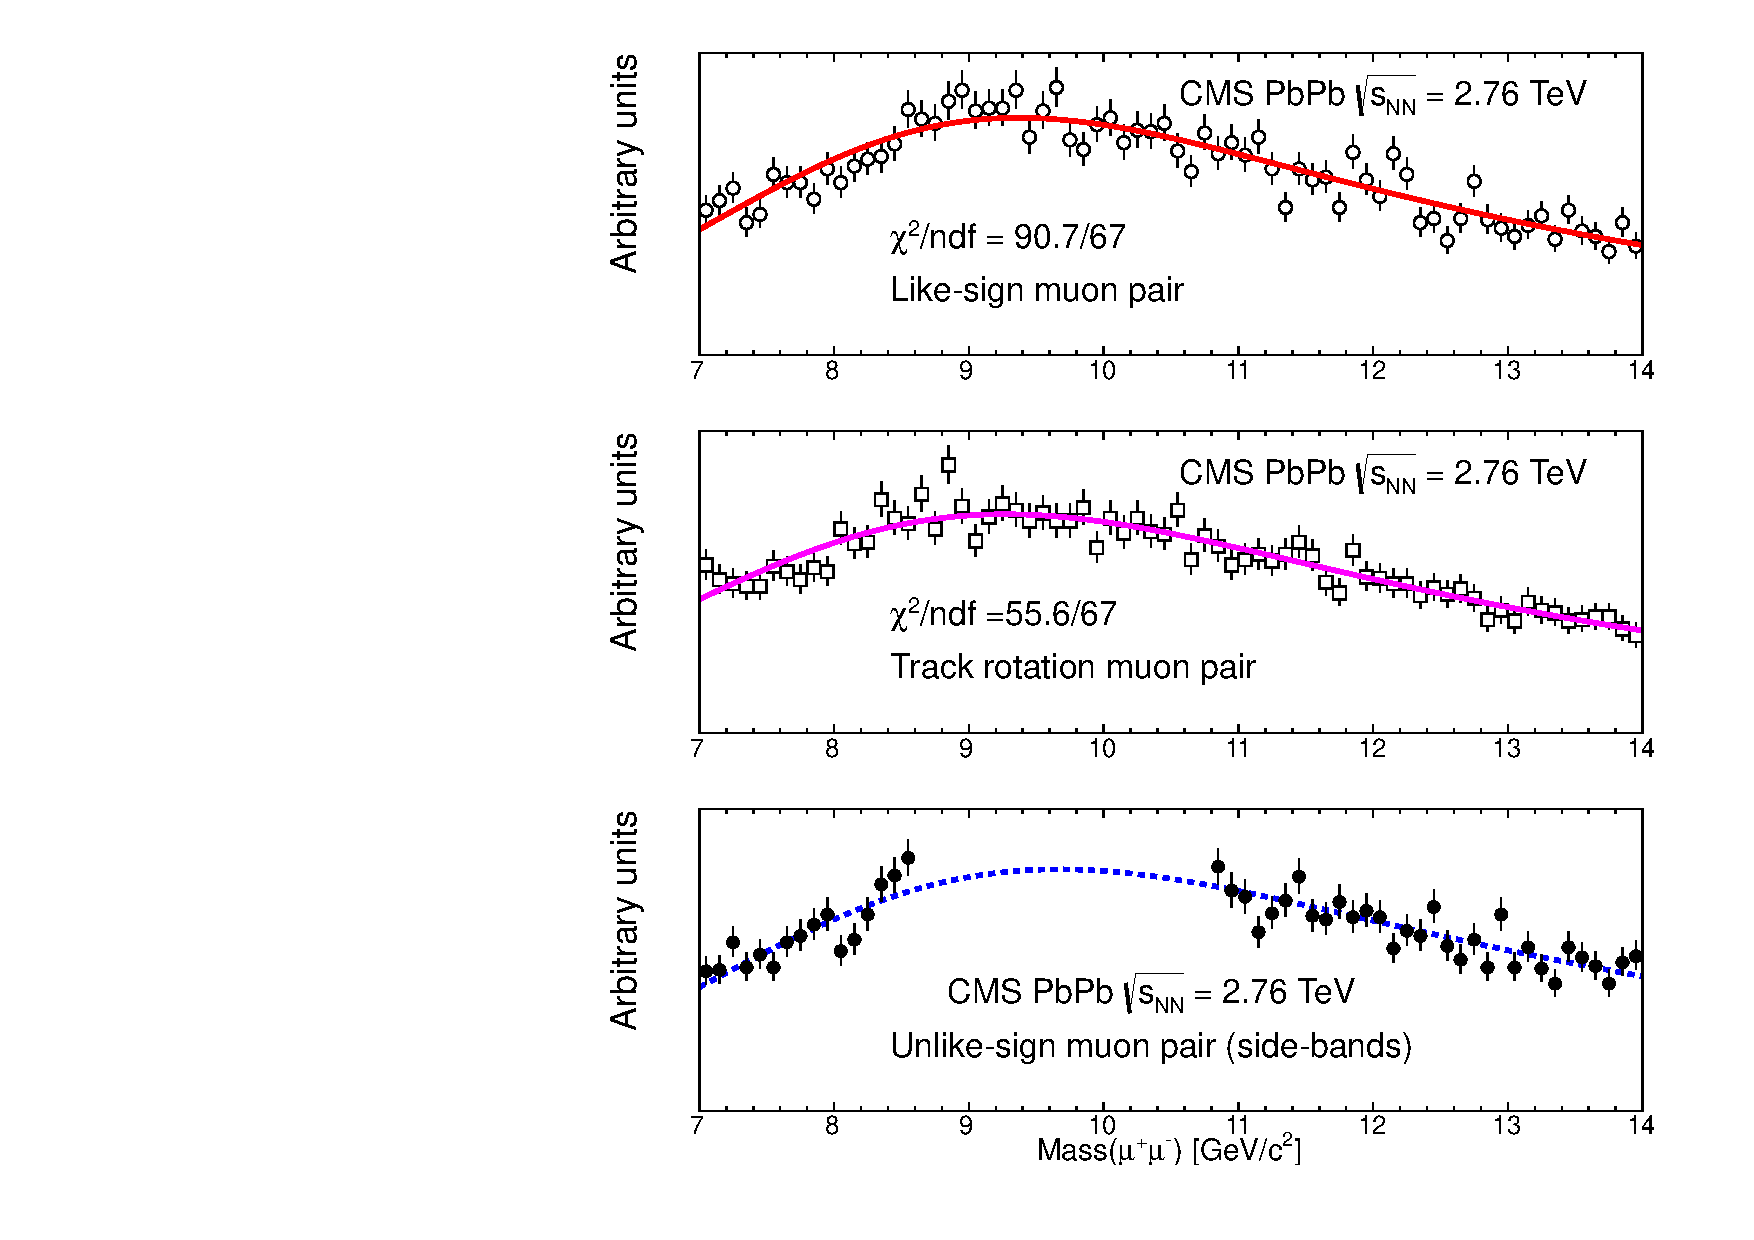
\includegraphics[angle=0,width=0.6\textwidth]{figures/fitting/plot3canvas.pdf}
    \caption{Compare like-sign, track rotation, and unlike-sign pairs}
    \label{fig:compareBkgd}
 \end{center}
\end{figure}

\subsection{Fits to the pp data}

The \pp 2.76 TeV dataset is the same as employed in the previous measurement~\cite{prl}. 
The same background fitting model as employed therein is adopted as nominal for the \pp case: 
second order polynomial. 

% https://espace.cern.ch/cms-heavyion/upsilon/fitting/ppdata.aspx

The same fitting model as devised for the \PbPb dataset is applied to the \pp dataset as well, to probe stability.  
Fit results are shown in \fig{fig:massfits_pp_nominal_all} for the nominal background model (error function times exponential), 
and in \fig{fig:massfits_pp_likesign} for fits utilizing like-sign information. 
The results are displayed for the $\pt^\mu>3.5\GeVc$ and $\pt^\mu>4.0\GeVc$ selections, 
and for the cases where the signal shape parameters are left floating and are fixed to the PbPb results.  
%
Despite the excessive number of parameters of the background model, when applied to the limited-statistics \pp dataset, the fit results show a fair stability. 


\begin{figure}[hbtp]
  \begin{center}
    \subfigure[$\pt^\mu>3.5\GeVc$]{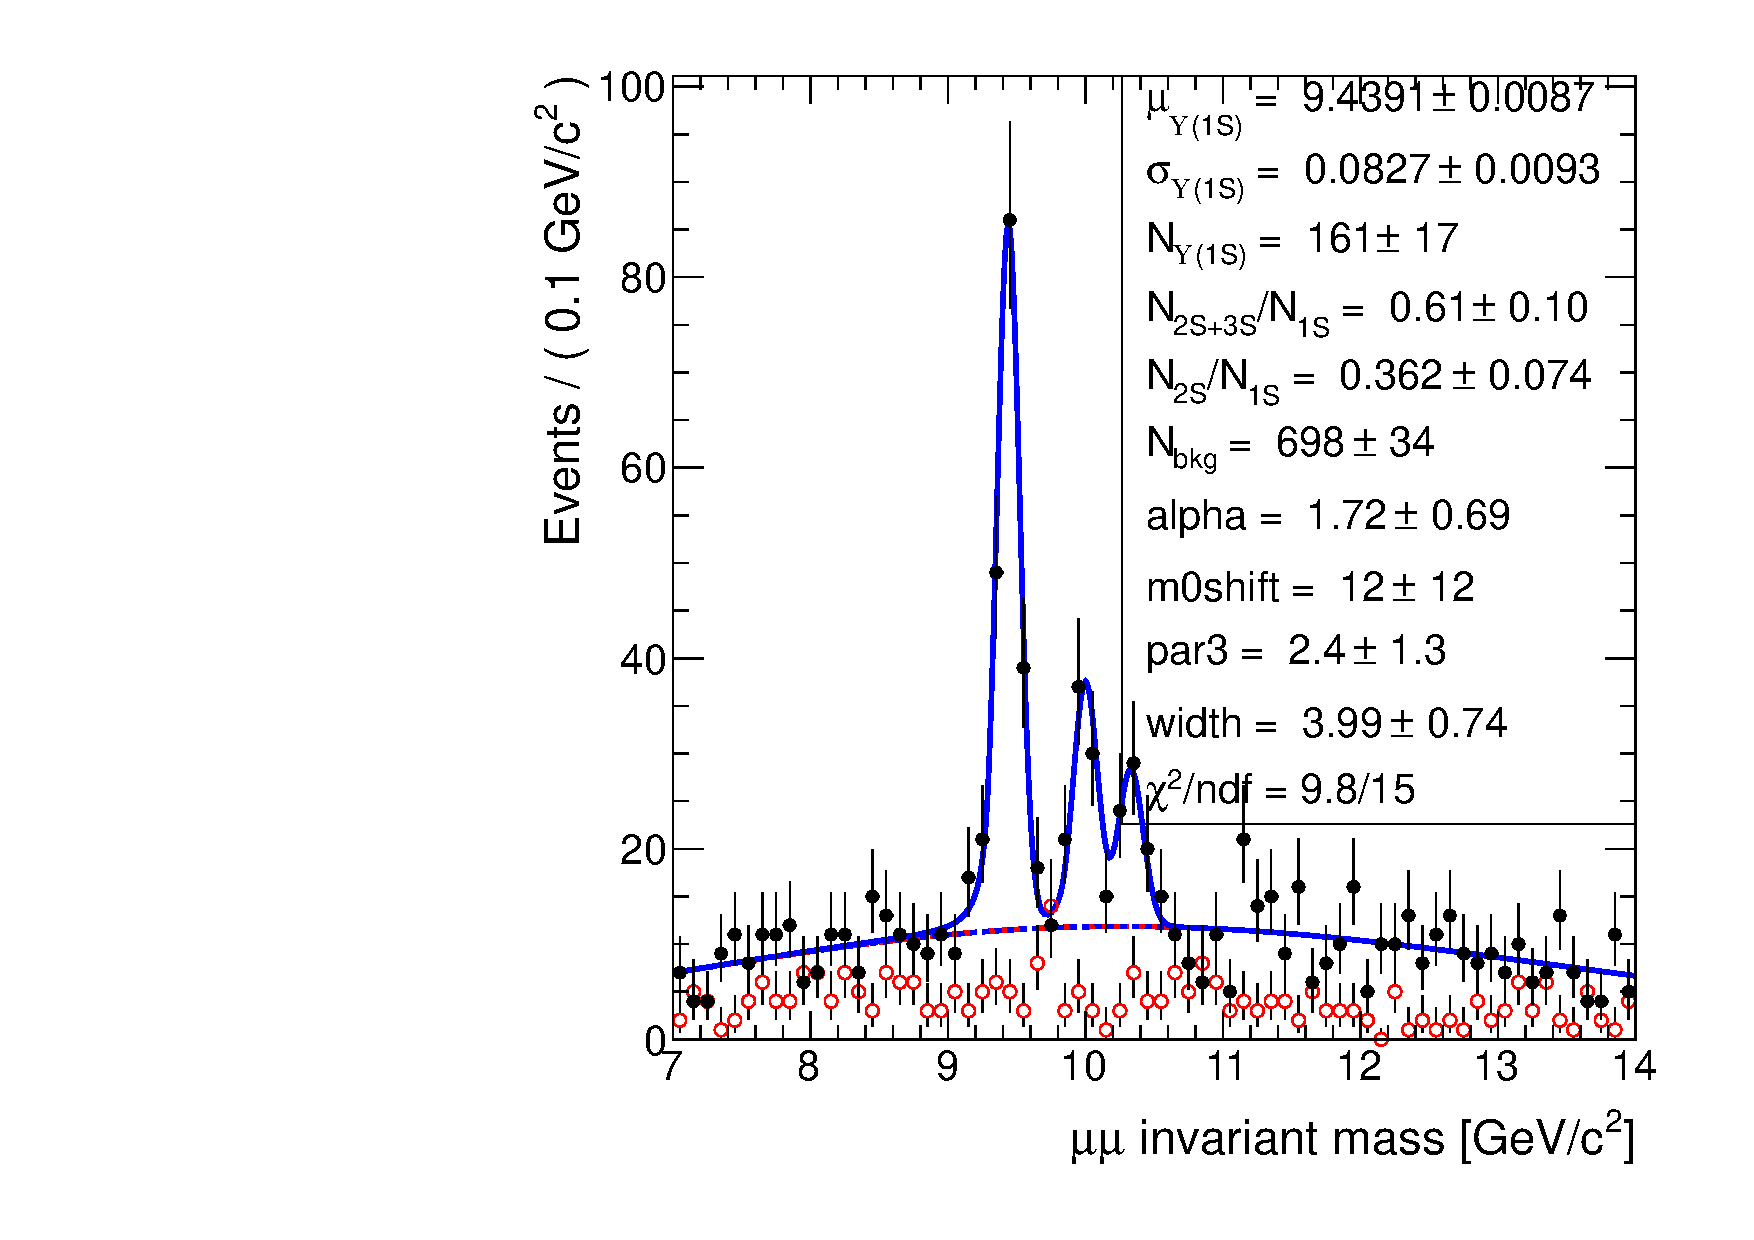
\includegraphics[angle=0,width=0.5\textwidth]{figures/pp276/masspeak_pp_HIrereco_erf_paramOn_MuonPT35}\label{fig:massfits_pp_nominal}}
    \subfigure[$\pt^\mu>4.0\GeVc$]{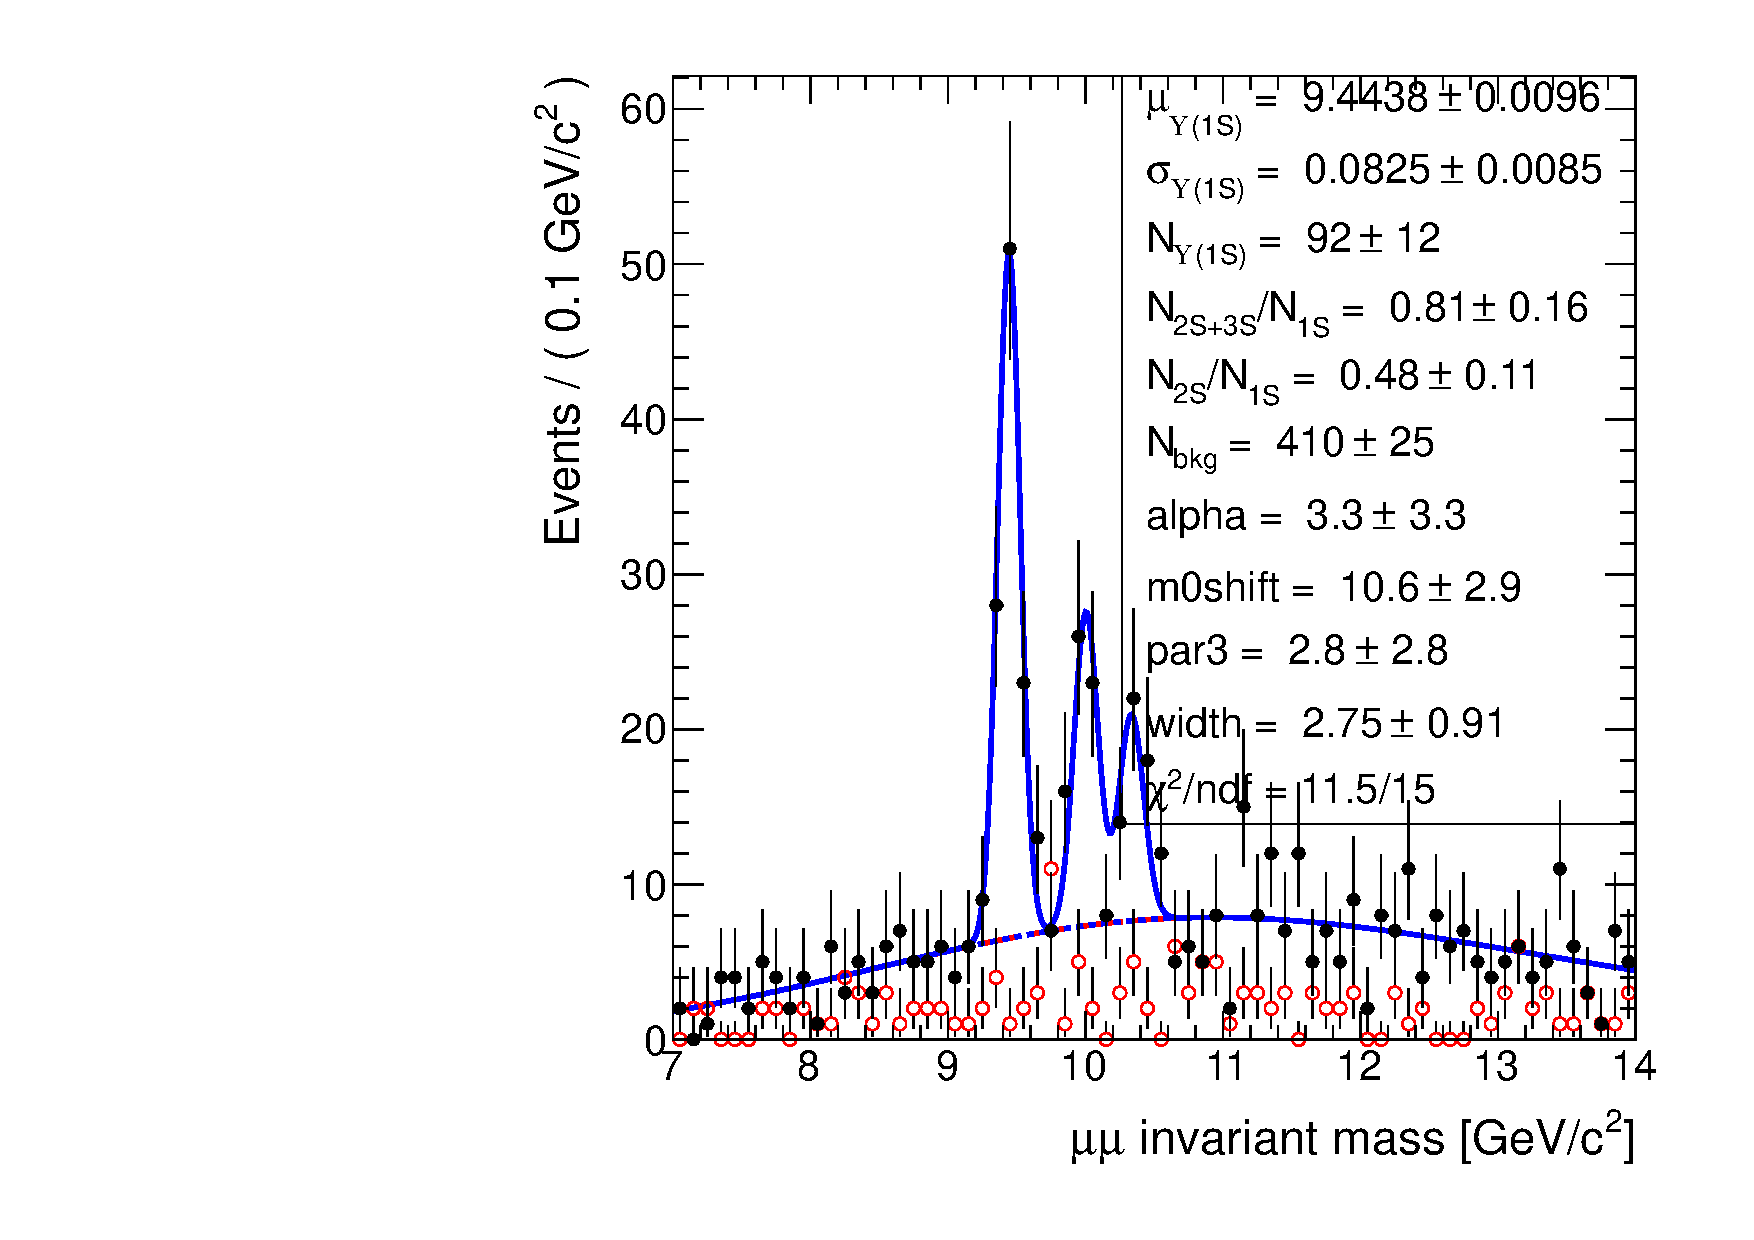
\includegraphics[angle=0,width=0.5\textwidth]{figures/pp276/masspeak_pp_HIrereco_erf_paramOn}\label{fig:massfits_pp_erf}}\\
    \subfigure[$\pt^\mu>3.5\GeVc$; signal shape fixed to PbPb]{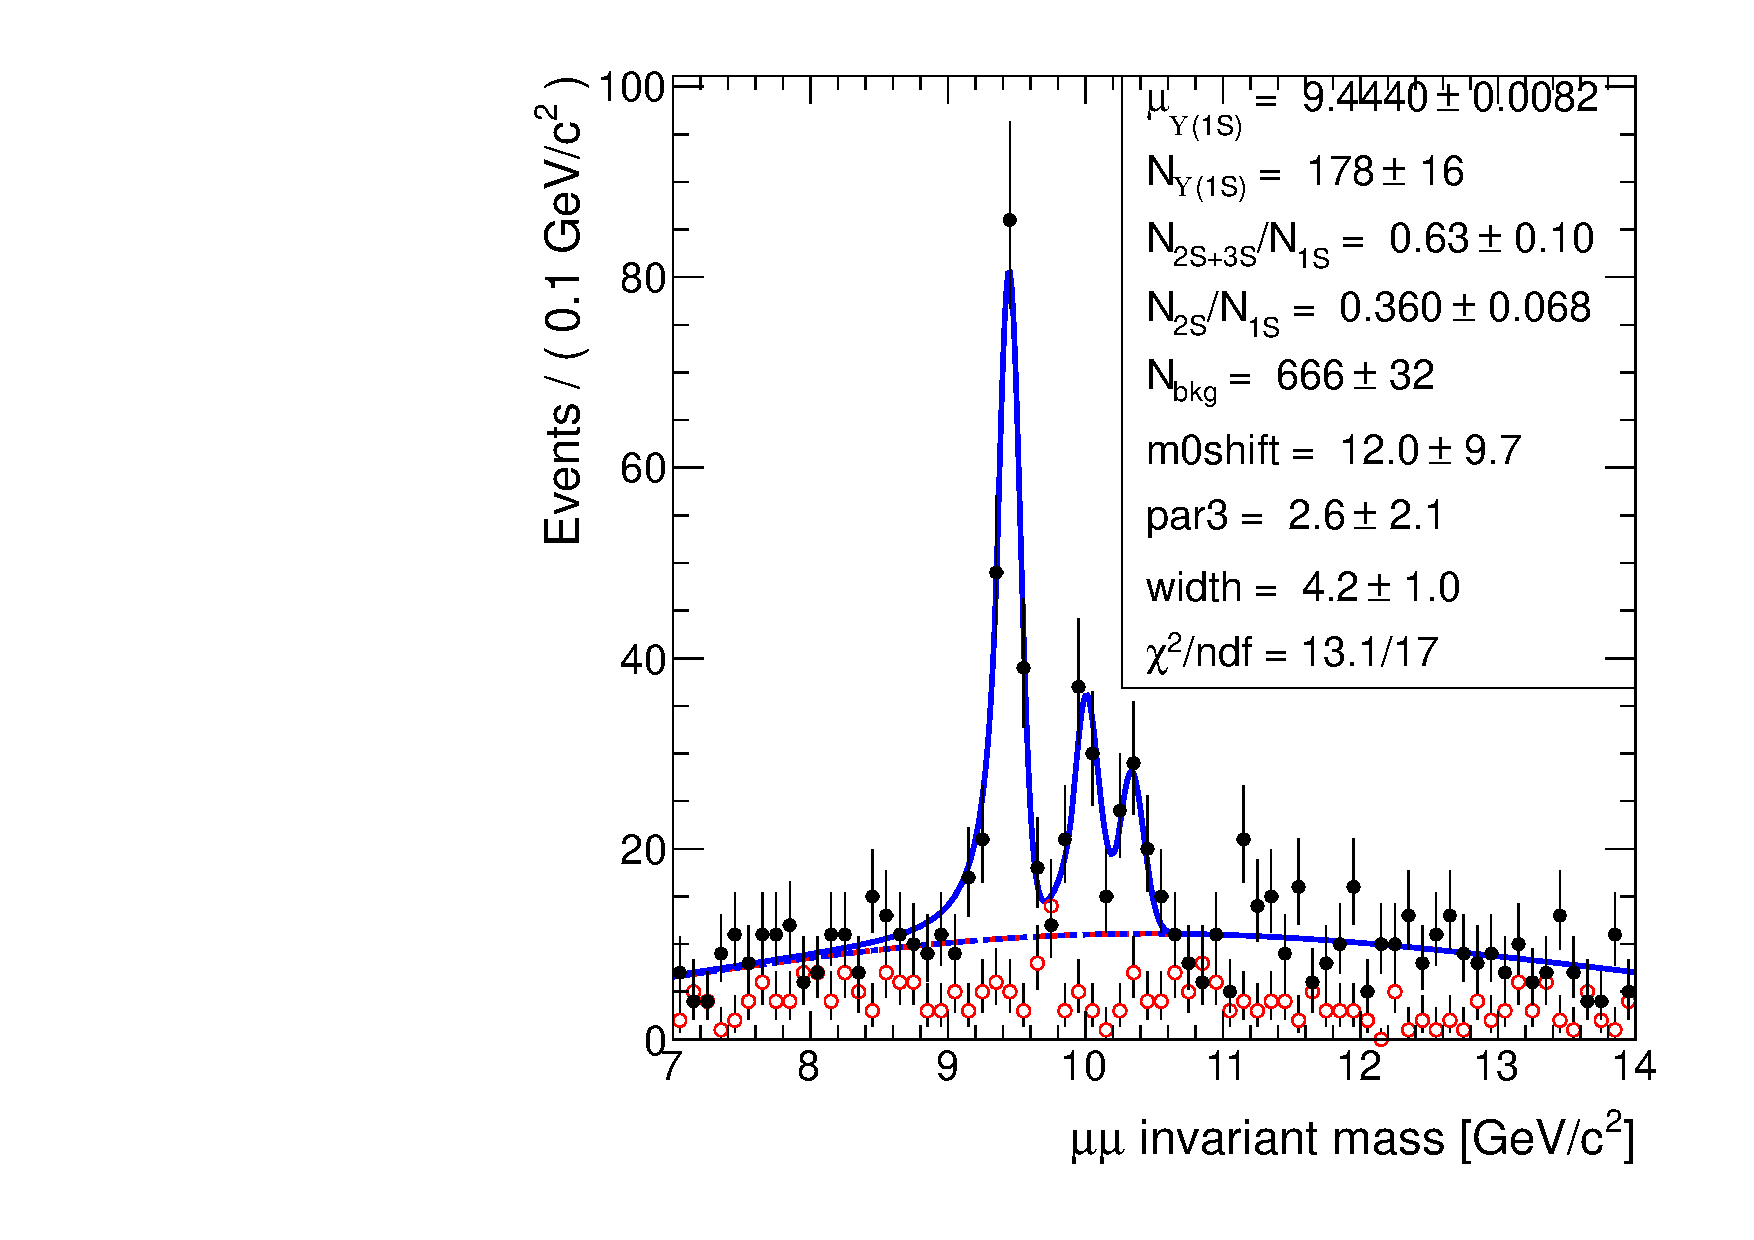
\includegraphics[angle=0,width=0.5\textwidth]{figures/pp276/masspeak_pp_HIrereco_erf_fix_paramOn_MuonPT35}\label{fig:massfits_pp_nominal_fix}} 
    \subfigure[$\pt^\mu>4.0\GeVc$; signal shape fixed to PbPb]{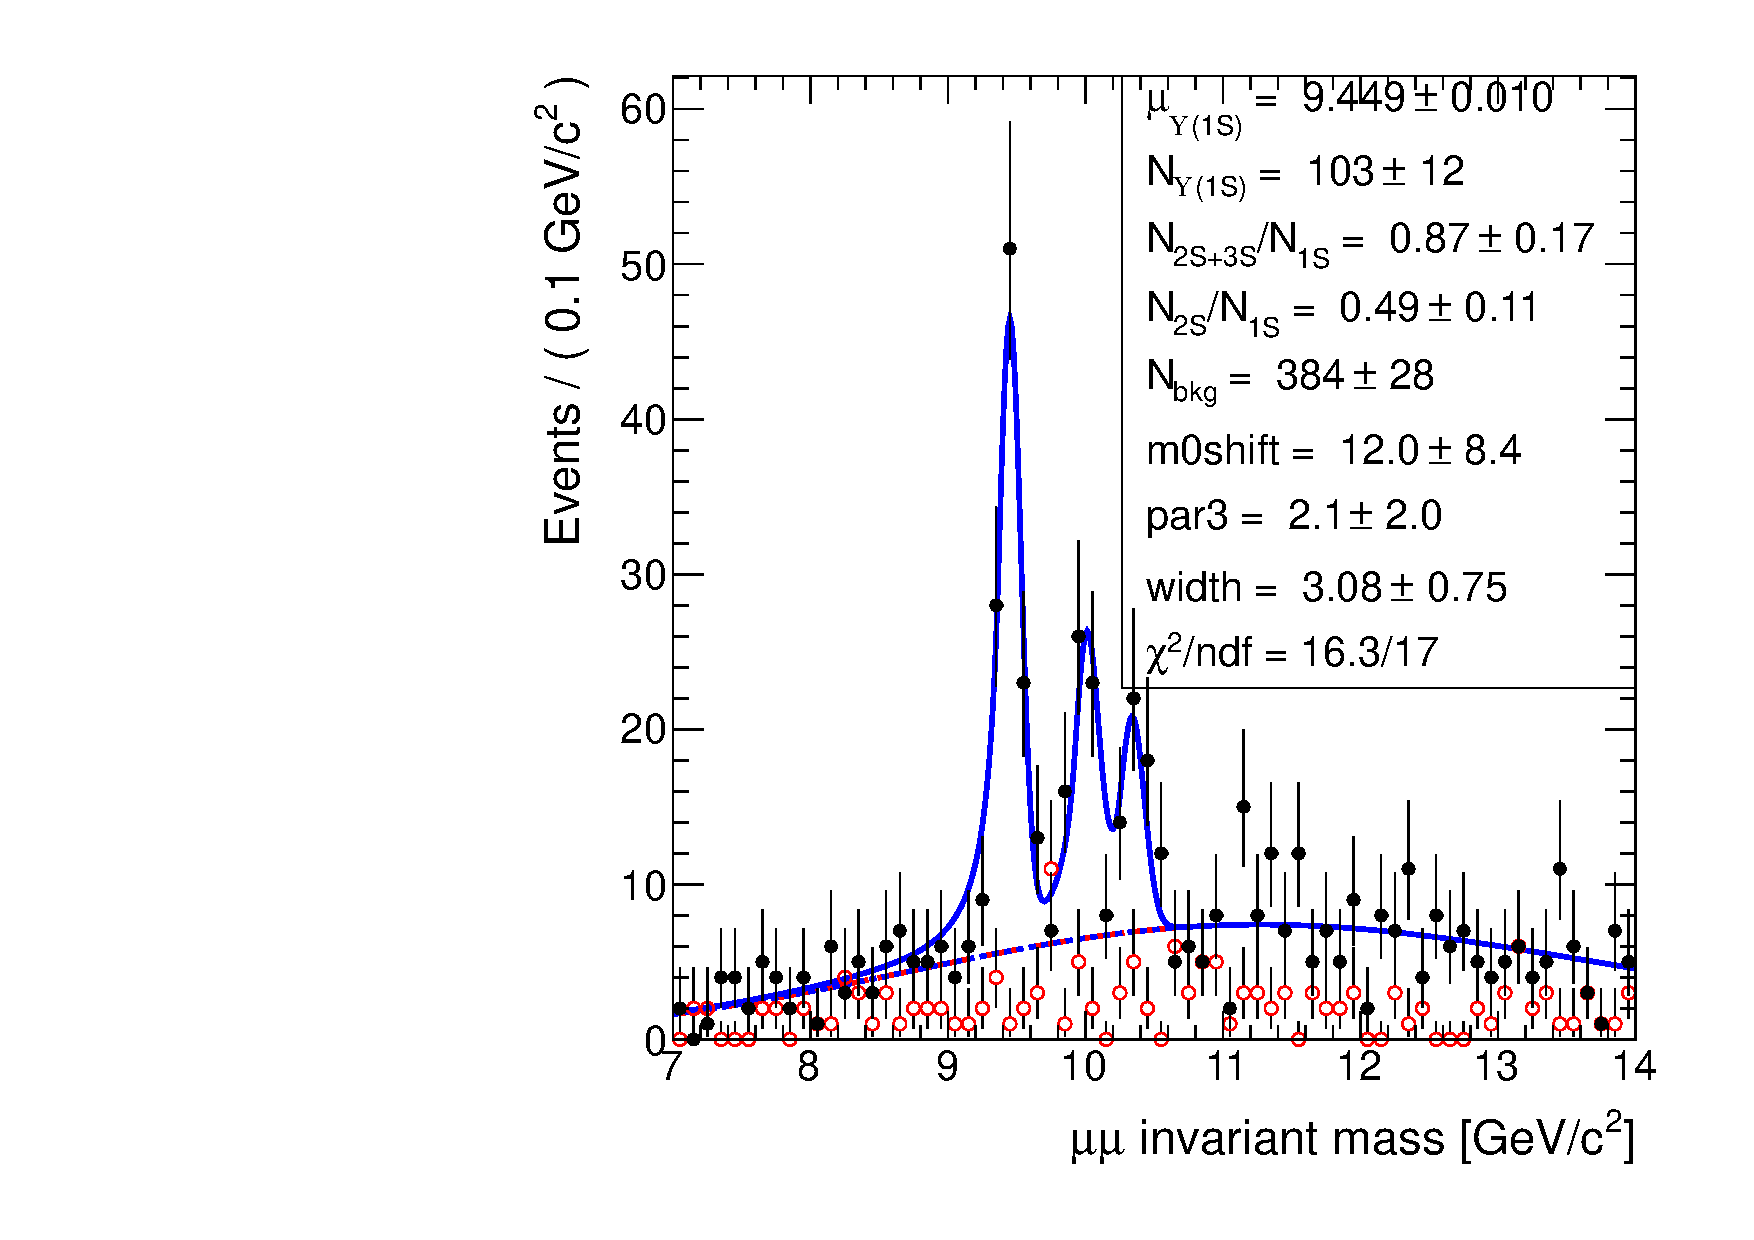
\includegraphics[angle=0,width=0.5\textwidth]{figures/pp276/masspeak_pp_HIrereco_erf_fix_paramOn}\label{fig:massfits_pp_erf_fix}}
    \caption{Mass fits to the pp data ($231 nb^{-1}$) with error function. Figs~\ref{fig:massfits_pp_nominal},~\ref{fig:massfits_pp_erf}: signal shape parameters are left floating; Figs~\ref{fig:massfits_pp_nominal_fix},~\ref{fig:massfits_pp_erf_fix}: signal shape parameters are fixed to the PbPb results.}
    \label{fig:massfits_pp_nominal_all}
  \end{center}
\end{figure}

\begin{figure}[hbtp]
  \begin{center}
    \subfigure[$\pt^\mu>3.5\GeVc$]{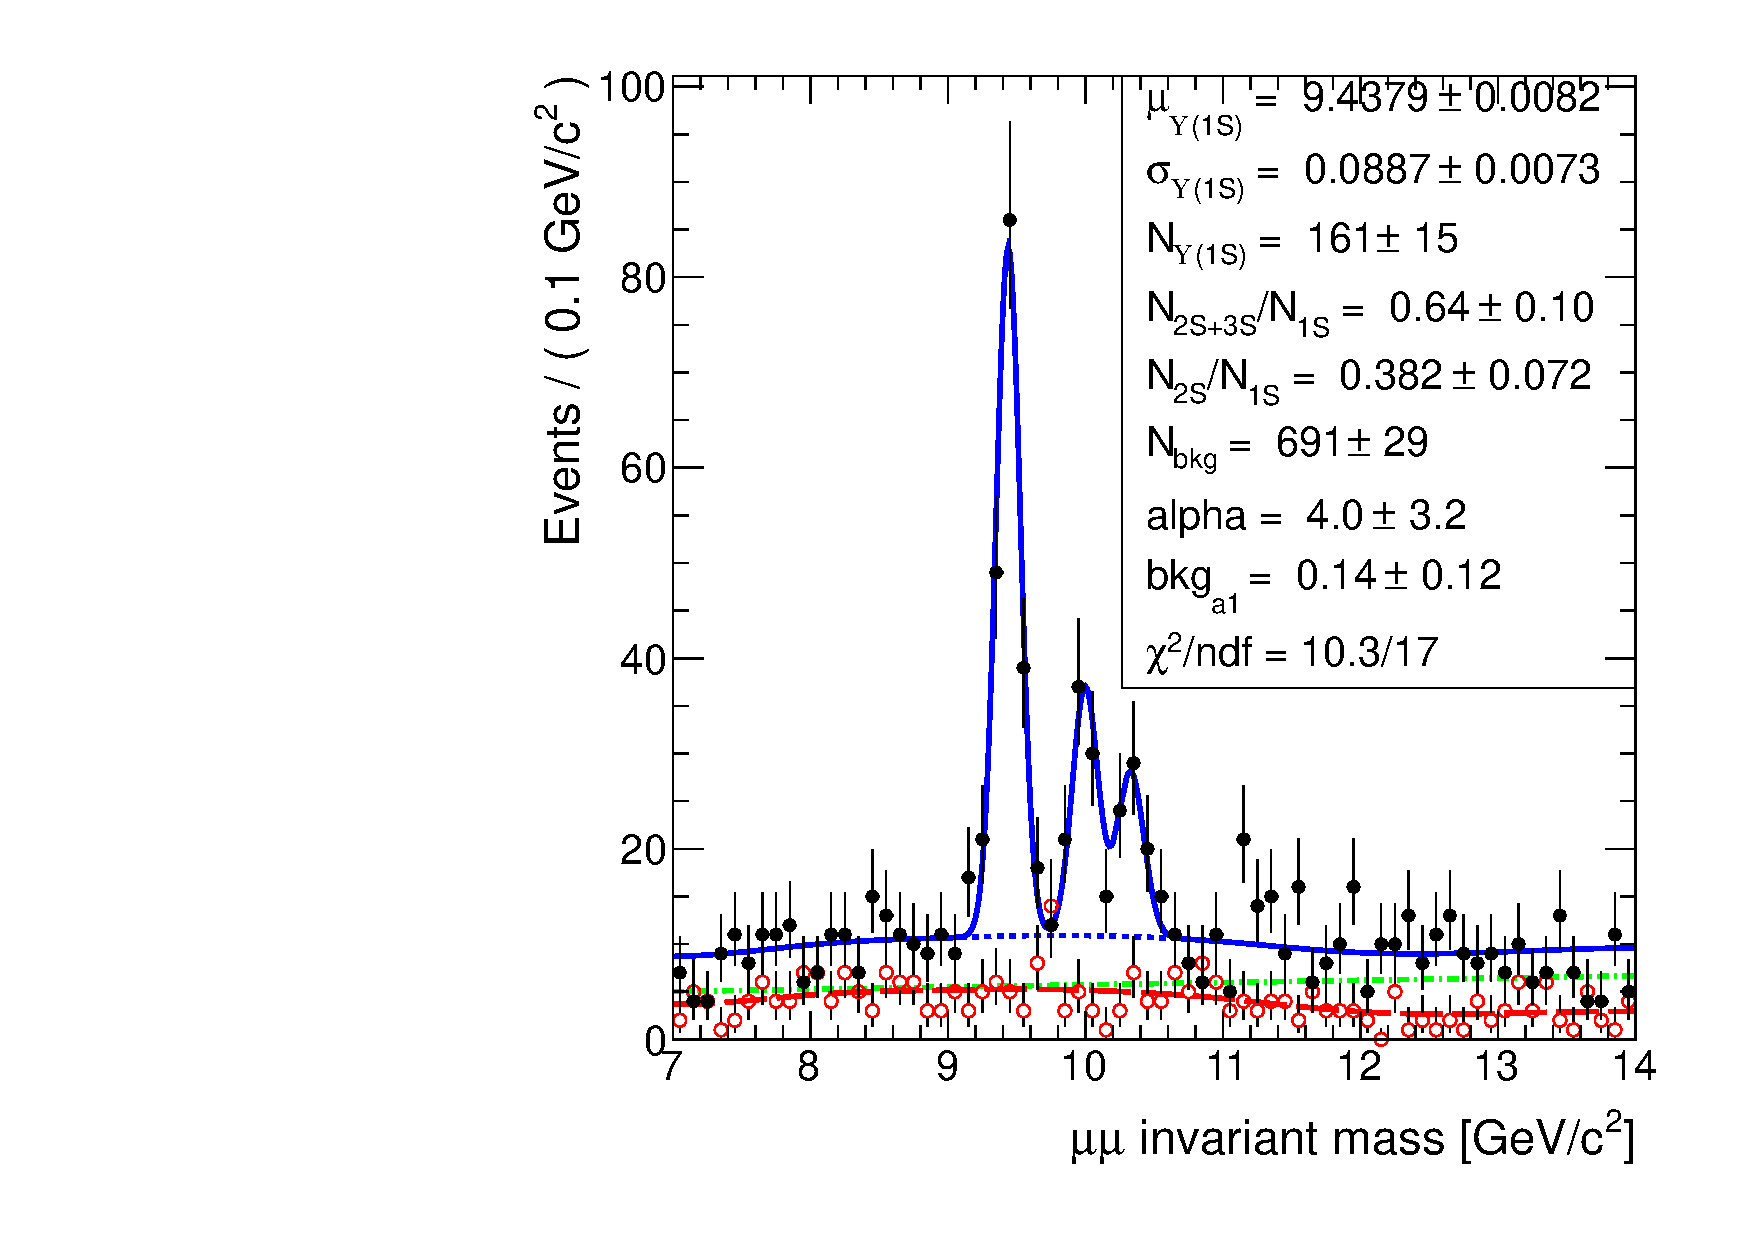
\includegraphics[angle=0,width=0.5\textwidth]{figures/pp276/masspeak_pp_HIrereco_paramOn_MuonPT35}\label{fig:massfits_pp_keys_35}}
    \subfigure[$\pt^\mu>4.0\GeVc$]{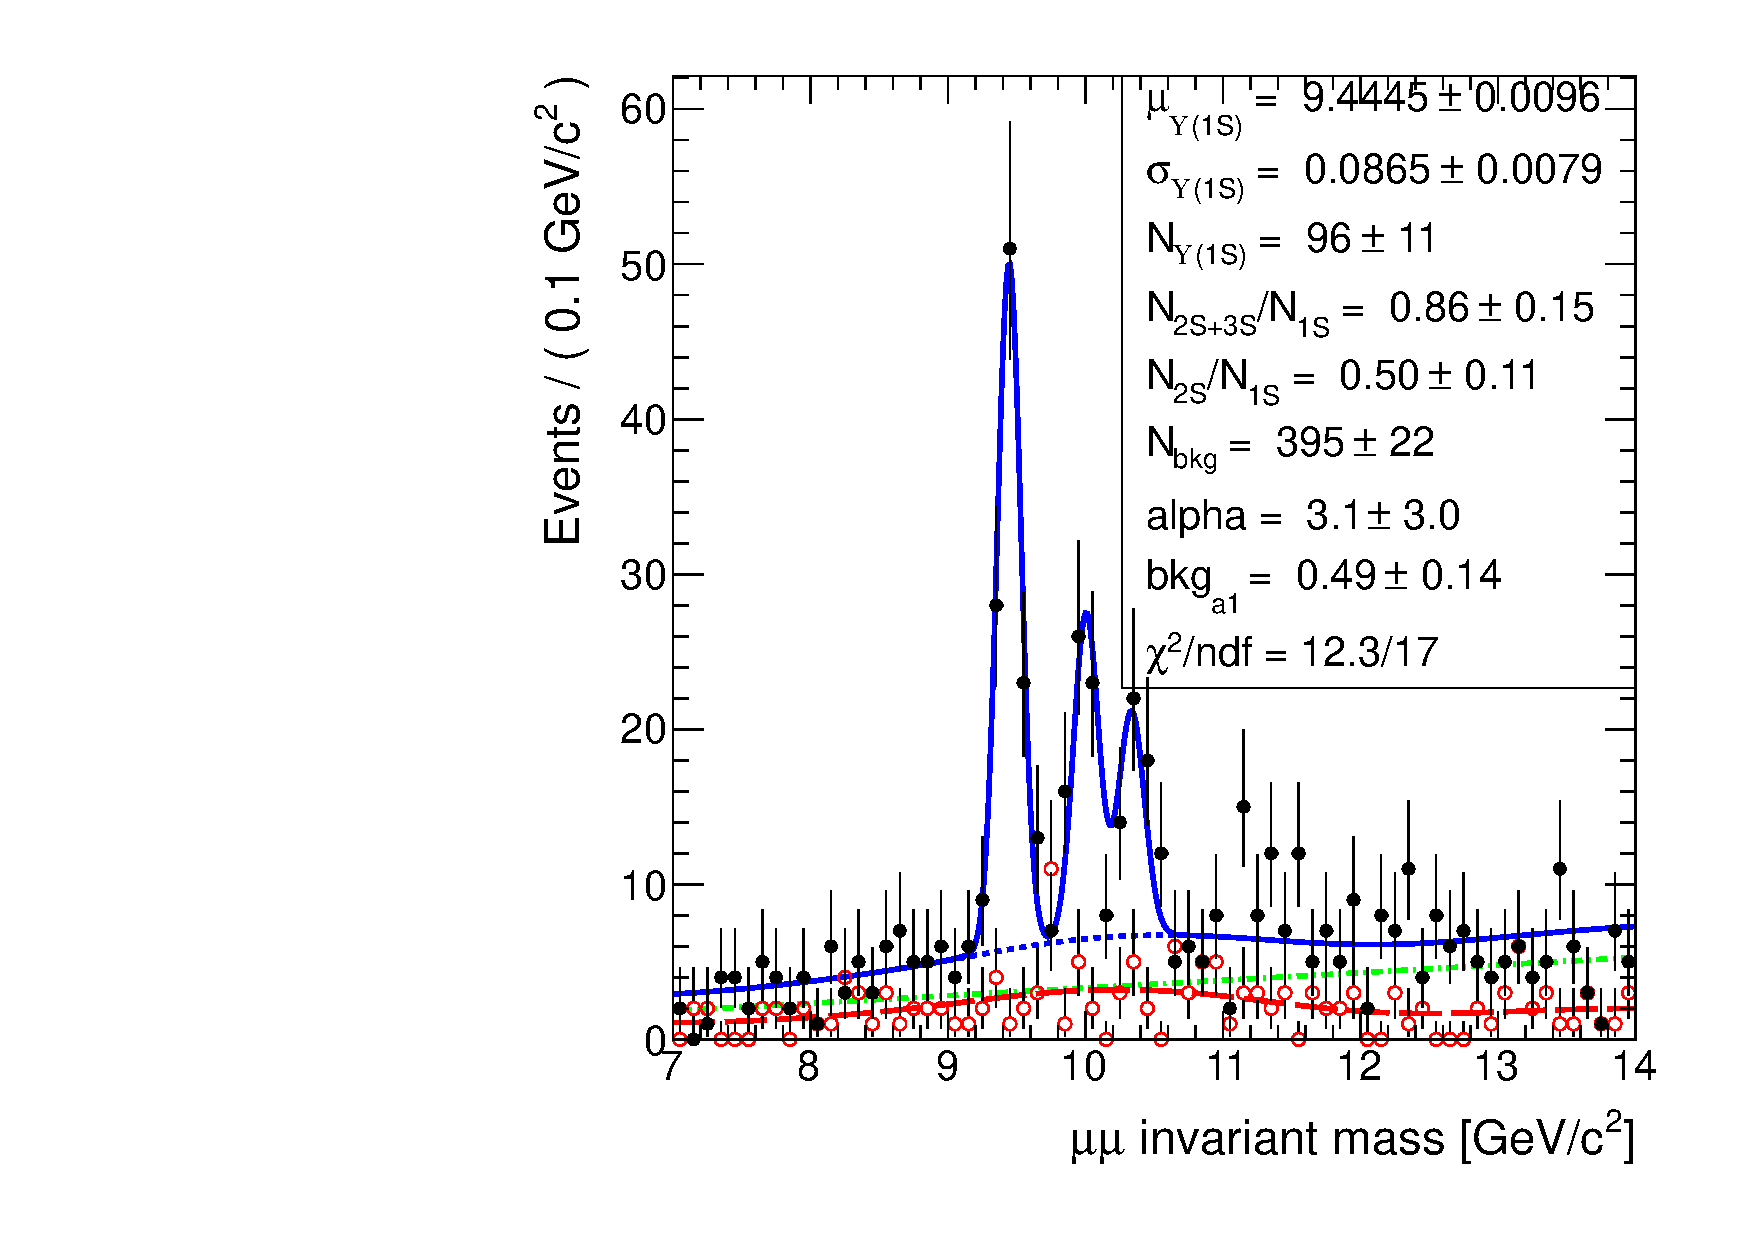
\includegraphics[angle=0,width=0.5\textwidth]{figures/pp276/masspeak_pp_HIrereco_paramOn}\label{fig:massfits_pp_keys}}\\
    \subfigure[$\pt^\mu>3.5\GeVc$; signal shape fixed to PbPb]{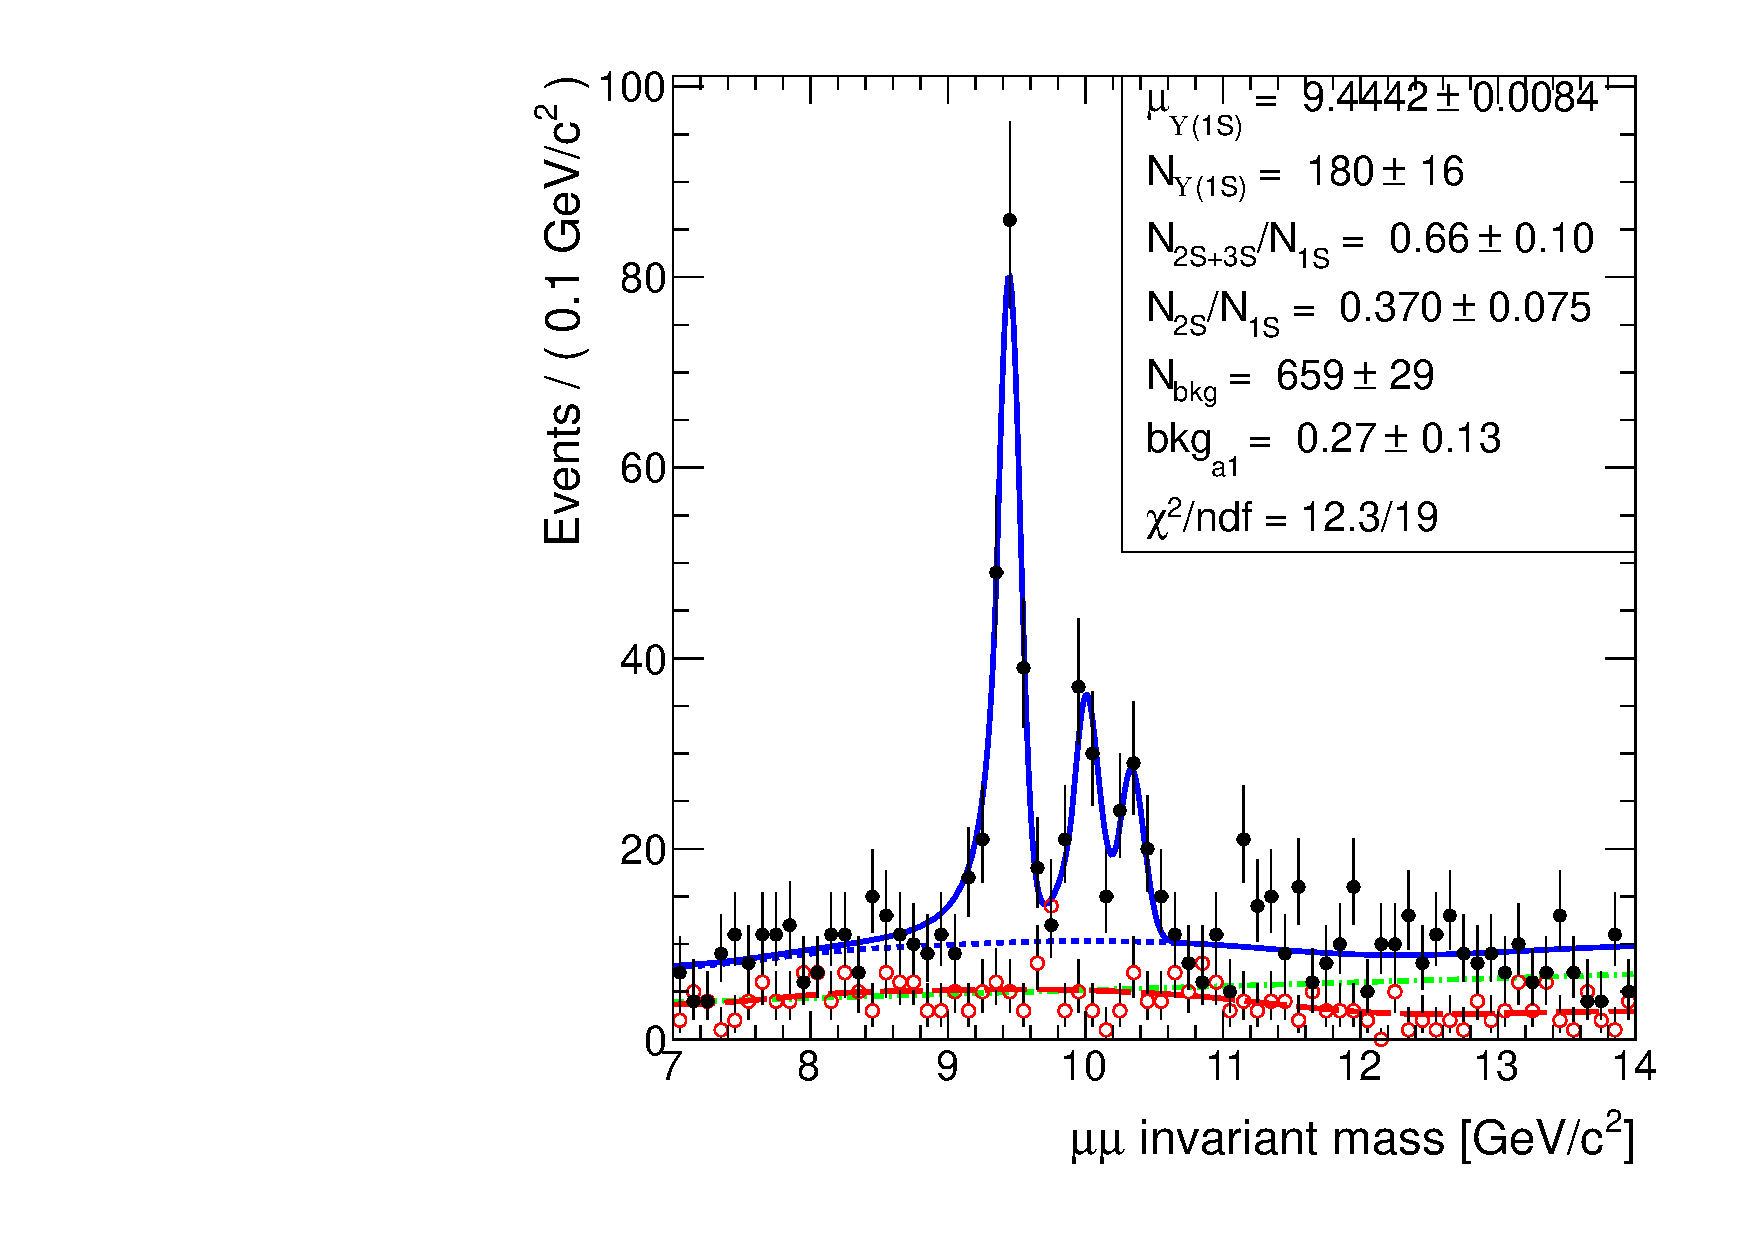
\includegraphics[angle=0,width=0.5\textwidth]{figures/pp276/masspeak_pp_HIrereco_fix_paramOn_MuonPT35}\label{fig:massfits_pp_keys_fix_35}} 
    \subfigure[$\pt^\mu>4.0\GeVc$; signal shape fixed to PbPb]{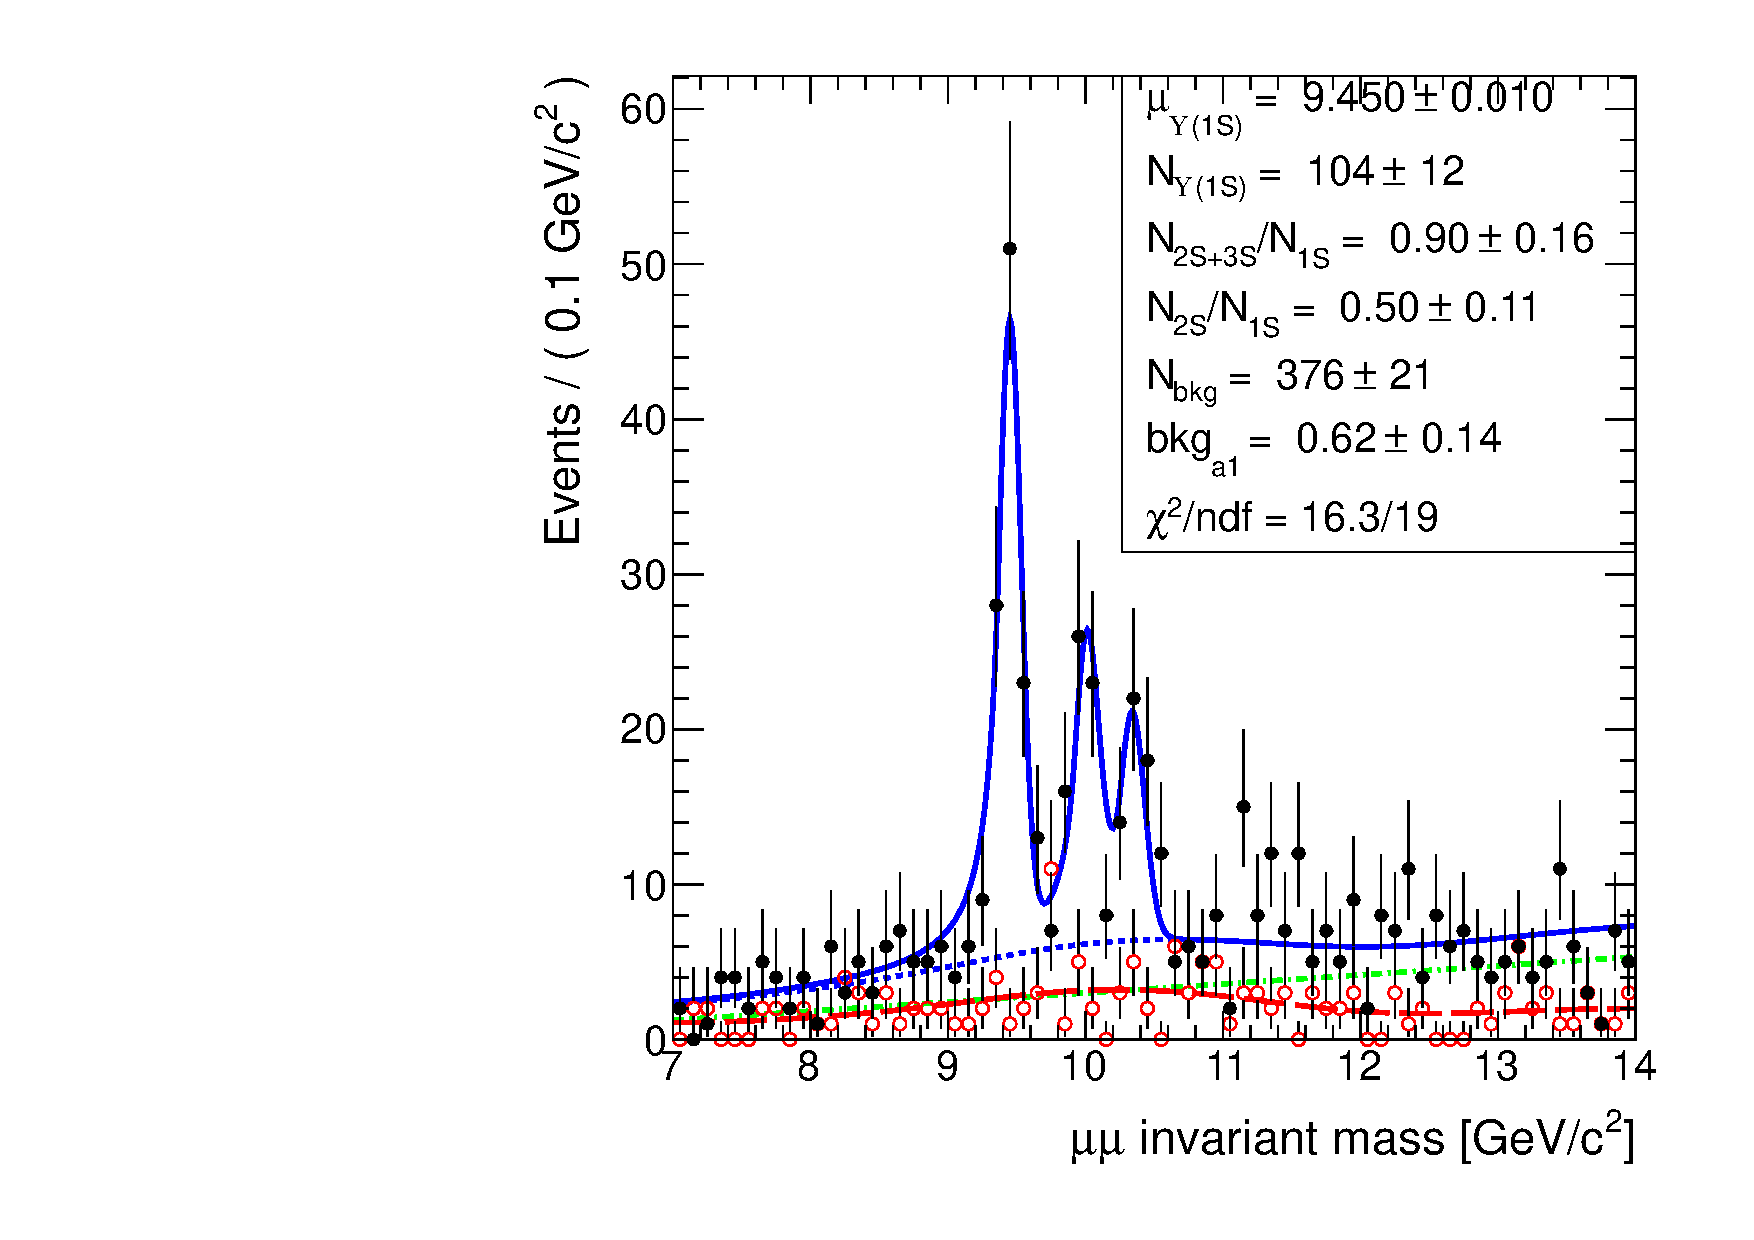
\includegraphics[angle=0,width=0.5\textwidth]{figures/pp276/masspeak_pp_HIrereco_fix_paramOn}\label{fig:massfits_pp_keys_fix}}
    \caption{Mass fits to the pp data ($231 nb^{-1}$), using like-sign information. Figs~\ref{fig:massfits_pp_keys_35},~\ref{fig:massfits_pp_keys}: signal shape parameters are left floating; Figs~\ref{fig:massfits_pp_keys_fix_35},~\ref{fig:massfits_pp_keys_fix}: signal shape parameters are fixed to the PbPb results.}
    \label{fig:massfits_pp_likesign}
  \end{center}
\end{figure}




%\subsection{Fits to the binned datasets}
%\subsubsection{Centrality dependence}
%(enter studies of mass resolution and fsr parameter dependence in MC and high-stat \JPsi data)

